%%%%%%%%%%%%%%%%%%%%%%%%%%%%%%%%%%%%%%%%%%%%%%%%%%%%%%%%%%%%%%%%%%%%%%%%%%%%%%%%%
%
%  Masterarbeit Christoph Neubauer 13.03.2017         
%  "Design and Implementation of a fault tolerant form processing application using machine learning"
%  Lehrstuhl fuer Mustererkennung, FAU Erlangen-Nuernberg
%
%%%%%%%%%%%%%%%%%%%%%%%%%%%%%%%%%%%%%%%%%%%%%%%%%%%%%%%%%%%%%%%%%%%%%%%%%%%%%%%%%

% ++ LME LateX Dokument 
%    Die Verwendung der option "german" bindet german.sty ein.
%    For english papers, use the "english" option and talk to your advisor.
%\documentclass[german,mt]{lmedoc}
\documentclass[english,mt]{lmedoc}

% ++ Umlaut Unterstuetzung
%    Paket "inputenc" kann verwendet werden, um z.B. Umlaute oder das scharfe S
%    direkt (als Nicht-ASCII-Zeichen) einzubinden. Dabei auf die korrekte
%    Kodiermethode achten (z.B. Linux: latin1)! 
\usepackage[latin1]{inputenc}

% ++ es werden keine underfull hboxes als Fehler ausgegeben,
%    da das ja nur heißt, dass die Seite noch nicht ganz voll ist
\hbadness=10000



\includeonly{mt01, mt02, mt03, mt04, mt05, mt06, mt07, mt08, mt09, mt10, mt11, mt-lit, mt-lof, mt-lot}

\pagenumbering{roman}

%\bibliographystyle{galpha1a} %german bibliography
\bibliographystyle{alphamod} %english bibliography

\def\ZweitInstitut{
Universidade Federal do Parana

 Curitiba}

\begin{document}
\clearpage
  \begin{deckblatt}
    \Titel{Design and Implementation of a fault tolerant form processing application using machine learning}
    \Name{Neubauer}
    \Vorname{Christoph}
    \Geburtsort{Homburg (Saar)}
    \Geburtsdatum{23.06.1991}
    \Betreuer{PD Dr.-Ing. habil. Peter Wilke}
    \ZweiterBetreuer{Prof. Luiz Eduardo S. Oliveira}
    \Start{12.09.2016}
    \Ende{13.03.2017}
  \end{deckblatt}

\cleardoublepage


Ich versichere, dass ich die Arbeit ohne fremde Hilfe und ohne Benutzung
anderer als der angegebenen Quellen angefertigt habe und dass die Arbeit
in gleicher oder "ahnlicher Form noch keiner anderen Pr"ufungsbeh"orde
vorgelegen hat und von dieser als Teil einer Pr"ufungsleistung
angenommen wurde. Alle Ausf"uhrungen, die w"ortlich oder sinngem"a"s
"ubernommen wurden, sind als solche gekennzeichnet.
\\

Die Richtlinien des Lehrstuhls f"ur Studien- und Diplomarbeiten
habe ich gelesen und anerkannt, insbesondere die Regelung des
Nutzungsrechts. \\[15mm]
Erlangen, den \selectlanguage{german} \today \hspace{6.0cm} \\[10mm]

\selectlanguage{english} %remove this line for german style

\cleardoublepage

\begin{center}
\bfseries
"Ubersicht
\normalfont
\end{center}


\vspace{5.0cm}

\begin{center}
\bfseries
Abstract
\normalfont
\end{center}

\cleardoublepage

\tableofcontents

\cleardoublepage \pagenumbering{arabic}

%%%%%%%%%%%%%%%%%%%%%%%%%%%%%%%%%%%%%%%%%%%%%%%%%%%%%%%%%%%%%%%%%%%%%%%%%%%%%%%
%
% Introduction
% 
%%%%%%%%%%%%%%%%%%%%%%%%%%%%%%%%%%%%%%%%%%%%%%%%%%%%%%%%%%%%%%%%%%%%%%%%%%%%%%%

\chapter{Introduction}
\label{cha1}
% 5-8 pages
% Some general information on the context and setting.
Optical Character Recognition (OCR) has been the topic of research for many decades. 
Several workshops, papers, and journals have been published, conferences hold on issues in this field. %irrelevant, ferner keine Quellen angegeben. Wuerde eher so heranfuehren, dass es ein 'active field of study' ist
%While there are still many open problems (for instance the accurate recognition of arabic texts, symbols, mathematic formulas or handwriting), the knowledge in this area has already led to the development of several highly accurate systems (especially based on English text).
Recent results have already spawned/created some highly accurate systems, especially based on English text. Currently, research focus is gradually shifting towards the recognition of non-latin alphabets and scalable approaches at OCR. %TODO:Hier ggf. noch nachlegen mit 'this thesis presents one such scalable approach ...'

%While already a lot of companies use those systems, there is still a majority of others that do not. But, as these systems grow more accurate each year, it is very likely that the need for ocr systems will grow. \par
While some companies are already using ORC as a means of process optimization, others have left its potential untapped. With more and more research towards scalable approaches, the demand for OCR systems is likely to grow in the future \cite{Klein04}\cite{Attaran01}\cite{Billentis16}.

As companies are getting connected and globalized, more and more data has to be handled. Modern keywords such as 'Big Data' or 'Data Mining' show, that there is currently a need for solutions to process that information.

One that offers increased optimization potential is invoice management. Companies all over the world have to manage not only the invoices they generate but also the ones they retrieve, e.g. from their suppliers.
Although ERP-systems capable of invoice generation already exist, they often represent specialized solutions that are not capable of handling foreign invoices. In addition to that, especially small but also medium-sized companies are mostly not able to afford such systems. 
% While there are already ERP-systems such as SAP ERP 6.0 that are capable of the generation of invoices, especially invoices of other companies are not that easy to process due to the differences between those documents. In addition to that, especially small but also medium-sized companies are mostly not able to afford such systems. 

In order to facilitate and accelerate the process of invoice recognition, electronic invoice formats have been introduced. If invoices are sent in such a format, a company recognizes the required fields and handles this invoice. Again, this is often the case for big companies, that have defined contracts with their suppliers or customers and have therefore been able to define an electronic invoicing format to automatically process an invoice.

For every other company, the problems persist: Not every invoice is sent in an electronic format, some are still sent as a normal PDF document or even postal.

\section{Motivation}
\label{sec1.2}
%Specific motivation for the problem at hand.

At the moment, invoices exist that do not meet any electronic invoicing standard. Due to the efforts made in regards to digitalization and standardization, it is to be expected that such formats will be a future standard for all invoices to be sent. But, although a variety of possible formats have already been defined electronic invoice still lacks one central standardized format.
%But even though electronic invoice formats have already been introduced, there are still a variety of formats and no real standard defined. 
Therefore, depending on the country or area, different formats are used. To address this issue inside the European Union, the E-Invoicing Forum of Germany (FeRD) developed a new format which will be very likely a new de-facto standard for companies inside the European Union. Small and medium sized companies can make use of this format as well as bigger companies. Chapter 2 will explain the different levels of the format more deeply.

While hardware parts and devices improve over time, we are now at a point were even personal computers are able to run complex calculations in lesser time. With this in mind, it would be a profit to automate invoice processing, even for small companies. Invoices that are processed manually do not only need employees but also much more time and are (due to the human factor) error-prone. Nevertheless, hardware parts can still be the limiting factor when it comes to performance.

With the use of machine learning techniques, it should be possible to develop an application that works on a personal computer, can handle lots of invoices and transforms them into an electronic invoice format.

\section{Task}
\label{sec1.3}

The task of this master thesis is to develop an application which can handle various invoices that are present in PDF format, extract necessary invoice information and transform and store those invoices enriched by the electronic invoice format. The advantages and disadvantages of this format should be evaluated first.
During the processing of the invoice, optical character recognition should be used to extract the information from the file. This process is supported by Machine Learning to provide additional analytical benefits.
Error-handling during the scan process is a task of the application.
The stored invoices should be retrievable again, enhanced and conform with the electronic invoice format, so that it is possible to process them further.

\section{Related Work}
\label{sec1.4}
This section will present other work and concepts that have been presented before and distinguish between their solution and the method used in this thesis. In addition to that, we will explain reasons why the presented approach has not been suitable for our solution.

\subsection{Case-based-reasoning on invoice documents}
The process of information extraction on invoice documents has been topic of research for many years. One approach using Case-based-reasoning (CBR) has been published by Hamza et. al. \cite{hamza07}. They present a two iterative step that first tries to classify the invoice document as a whole (global-solving) and later repeats the classification on a keyword and pattern structure level (local solving). Keywords in this approach are invoice specific words, such as the issue date or invoice number. Pattern structures are words that appear in tables. An invoice always has to list every single position, thus the preferred way to do this is using a table in a document.
The case-based reasoning approach is an iterative approach that stores information if a pattern structure has been found on the same line or the same column and if the relevant data is present before (over) or after (under) the keyword. This way cases are stored in a database and reused every time a new invoice has to be classified. The global solving resulted in an accuracy of 85.29\% whereas the local solving yielded 76.33\%.
%TODO: Write how we do it and negative things of CBR
\subsection{Using a predefined layout}
Another approach that has been presented by Cesarini et. al. is a definition of a structure how invoices look alike \cite{Cesarini98}. This model has to be created by a user before and can be seen as a template. The system knows on which positions relevant invoice information are, due to the predefined locations from the template.
Some of the scanned invoices may contain quality issues (e.g. have been scanned with an angle) that have to be taken into account while processing the document. Counteractions, such as deskewing\footnote{Deskewing is related to the rotation of an image to a zero degree angle} the invoice document, have to be applied in a way that the template can be applied on the document.

We are not using a predefined layout that has to be manually created by the user. Instead, the application will learn from the position of keywords in previously processed invoice documents and reuse this pattern on invoices documents of the same creditor.

The major downside of the approach of Cesarini et. al. \cite{Cesarini98} is the need of a manually created template. This does not only take time and is error-prone, but also only applies on invoices of exactly the same structure. But, especially in the field of invoice documents, there are various kinds and different structured invoices. This would lead to the expectation, that the user has to create a template every time an invoice of a new customer, supplier, etc. should be processed.

\subsection{Extracting information from repeated text}
Another issue to deal with invoices is to extract every position that is listed in the invoice. Typically these are multiple positions and therefore displayed in a table. A paper by Bart \& Psarker \cite{Bart10}  describes an approach that recognizes repeated structures by analyzing the basic similarity between lines, the separation, as well as gaps in between, to find out the relevant information.

In the application presented in this thesis, a histogram is used to detect tables which contain information. This enables us to narrow the relevant words to the ones inside the table. In addition to that, keywords that either mark table header words or sum up the positions at the end of the table are filtered out.

The approach of Bart \& Psarker \cite{Bart10} is based on the assumption that there are multiple lines of positions. Although this is often the case, there are also invoices with only one position that would not be detected. Also, other relevant keywords will not be detected if they are not presented in the invoice document as a table (or at least embedded in a repeated structure).
In our approach, we do not identify lines by calculating similarities or gaps. Instead, a search for table lines is made and position information are read that stand between starting and ending keywords.

%Other relevant academic work and how it differs from this work, for
%example %\citet{shannon_diff} and %\citet{blowfish}. Distinguish between
%``textual'' citation, as shown in %\citet{shannon_diff}, and
%``parenthesis'' citation %\citep{blowfish}.

\section{Results}
\label{sec1.5}
%What has been achieved in this work?
This thesis presents an application that is capable of automatic form processing and transformation of an invoice document into an electronic invoice format. The application makes use of the hOCR microformat originally presented by Thomas M. Breuel \cite{Breuel07} during the OCR process. This way the position of keywords are stored and can be reused when similar invoice documents should be processed.

A Machine Learning algorithm supports the extraction of invoice information. The relation between a position and a set of debit and credit accounts are saved. A Na{\"i}ve Bayes classificator is used to determine the most reasonable combination of credit and debit accounts for a new position.

Processed invoice documents are stored in the database and can be retrieved using a search function. All processed and saved documents are conformal with the ZUGFeRD standard originally published in 2014 \cite{Ferd14}.

\section{Outline}
\label{sec1.6}

%How is the thesis structured and why? 
This thesis is structured as follows: First, several electronic invoice formats are presented, explained and compared. Important criteria for the selection of a format are defined. These criteria will be applied to the formats in order to decide which format will be supported by the application.

After that, we will explain how we want to process a file to a document in the selected electronic invoice format. Chapter 3 will deal with OCR, the available systems at this time as well as a comparison between them and the selection of one of them (including the explanation why this selection has been made).
As the application should learn and improve results over time, we will also deal with machine learning techniques and choose an appropriate one. Chapter 4 will focus on this issue.

Chapter 5 will now discuss several use-cases of the application and show the architectural concept of the application. The following sections will deal with each module and explain it in-depth.

Finally, chapter 6 will conclude about this thesis. The accuracy of the application will be presented on generated data. The resulting application will be explained briefly again. Issues that are still open, as well as ideas that could improve the application, are listed.

\section{Acknowledgments}
\label{sec1.7}

During the implementation of the application and the creation of this document, several people helped me to achieve this presented work. I would like to thank some people in particular:

To Dr. Peter Wilke, who not only supervised my work but also put thoughts to things that I have not considered before but were crucial for the application.

To Prof. Dr. Oliveira, who supervised my work during my stay in Brazil and who gave me good input especially in the field of OCR.

To Prof. Daniel Weingaertner, who managed my stay in Brazil, enrolled me in the university and organized all the necessary documents.

To Daniel Stemler whose engagement enabled me to gain access to various invoice documents in order to get a reasonable amount of data to test on.

And to several other friends that helped me or supported me with advice or discussions about technologies or to clarify my understanding regarding a specific approach.   % 	Einfuehrung (\chapter{Introduction})
\cleardoublepage
%%%%%%%%%%%%%%%%%%%%%%%%%%%%%%%%%%%%%%%%%%%%%%%%%%%%%%%%%%%%%%%%%%%%%%%%%%%%%%%
%
% Electronic invoice formats - A comparison
% 
%%%%%%%%%%%%%%%%%%%%%%%%%%%%%%%%%%%%%%%%%%%%%%%%%%%%%%%%%%%%%%%%%%%%%%%%%%%%%%%
\chapter{Electronic invoice formats - A comparison}
\label{cha2}

During the digitalization of companies over the world, electronic invoices (also known as e-invoice) have become more and more important. E-Invoicing offers companies the possibility to improve their business processes, making invoicing faster and more efficient and enables a direct connection to other tools like ERP-Software. 

To give companies access to these benefits and to make the communication between companies even possible a comprehensive standard must be defined. With an invoice standard at hand, companies can use invoices from their business partners and read them into their systems (in the case of Business-to-Business (B2B)). 

Several invoice standards are currently used. The next section will deal with the most important ones and describes them as well as pointing out the benefits and drawbacks of the format.
After that, the next section defines criteria that are relevant for the application and how to measure them.
In the last section, these criteria are applied to the formats defined in section \ref{sec2.1} and compared against each other. Eventually, a decision regarding the usage of one of these formats is made.

\section{Description of leading formats}
\label{sec2.1}

Each of the following subsections will present an electronic invoice format. The history of the format, as well as the current version and, if found, the future promise will be explained. As there exist many different formats, it is out of the scope of this thesis to describe them all. %Instead, we will pick a few that we think are either important, promising or especially related to the region (Germany and the European Union).
Instead, we will pick a few that seem important and promising in regards to Germany's and the EU's demands towards an invoice standard. 

\subsection{UN/EDIFACT}
\label{sec2.1.1}

EDIFACT is a well-established \cite{basware} subset of standards from CEFACT regarding the electronic interchange of structured data. The word 'EDIFACT' is an acronym from 'EDI' which stands for 'Electronic Data Interchange' in combination with 'FACT' (for Administration, Commerce, and Transport). It is developed and maintained by the United Nations Economic Commission for Europe (UNECE) \cite{unece}.

The European Commission states that the UN/EDIFACT INVOIC message has been a 'cornerstone' in electronic invoicing over the past years \cite[page 14]{ec12}.

There are several subsets of EDIFACT that have been developed for different industries. For instance, the chemical industry uses CEFIC/ESCom\footnote{see also: \url{https://www.cefic.org/Industry-support/Implementing-reach/escom/}} as their standard, while automotive industry is in charge with ODETTE/FTP2\footnote{see also: \url{https://www.odette.org/services/oftp2}}.

EDIFACT has different message types such as \emph{ORDCHG} for a request to change an order or PAYORD which contains a payment order. In the context of this thesis, the message type \emph{INVOIC} (containing an invoice) is the most interesting one.

\subsection{XCBL}
\label{sec2.1.2}

The XML Common Business Library is an extension of the CBL which originally has been developed by Veo Systems Inc. \cite{coverpages}. The company has been bought by Commerce One Inc. in 1999 \cite{co}, page 29. 

xCBL currently exists in version 4.0 (since 2003)\footnote{see also: \url{https://www.xcbl.org}}. Since the company has gone bankrupt in 2004 \cite{scm} it is not very likely that this format gains more interest in the future.

\subsection{OASIS/UBL}
\label{sec2.1.3}

UBL stands for Universal Business Language and is being developed by OASIS. The current version is 2.1 and is normed by the international standardization organization\footnote{see ISO/IEC 19845:2015}.

Several countries developed their own subset of this format. Especially interesting in this case is a project called PEPPOL (Pan-European Public Procurement Online project) that aims at developing a format for public sectors in the whole European Union\footnote {see also: \url{https://www.peppol.eu/about\textunderscore peppol/about-openpeppol-1}}. 

Also interesting in the context of invoice interchange is the UBL-based project called \emph{simplerinvoicing} that aims at connecting ERP systems with accounting and e-invoicing software by providing an own invoicing standard\footnote {see also: \url{www.simplerinvoicing.org/en/}}. 

\subsection{ZugFerd}
\label{sec2.1.4}

This invoice format has been published initially in 2014 \cite{Ferd14}. The name is a german acronym, containing the name of the corresponding forum (FeRD). It can be translated to ''Central User Guide of the Forum for electronic Invoicing in Germany''. 

Although this invoice format is rather young it tries to fulfill the directive 2014/55/EU of the European parliament \cite{eu14} while still being flexible and simple. This directive states that the use of electronic invoice formats should be adopted by all member states of the European union until the 27. of November 2018 \cite[article 11]{eu14}. 
 
The approach of the ZugFerd-format enables not only big companies to work with that format, but also smaller and medium companies (SME's) that are in need of such a format but are normally not able to implement a complex electronic invoice standard. 
Furthermore, three levels of conformance are defined: Basic, Comfort, and Extended. Each of those levels has a different amount of required information fields, that have to be set in order to be valid. Nevertheless, in all of the three formats, it is possible to define more information in free text fields. 

This enables extensibility of the format and the possible business areas in which this standard can be used.

Based on the directive 2014/55/EU \cite{eu14} a bill draft has been developed by the federal government of Germany \cite[page 10]{br16} that suggests the usage of the ZugFerd standard to ensure interoperability. In addition to that, the federal association of energy market and communication (EDNA) also published a recommended course of action for the usage of the ZugFerd standard \cite{edna16}.

\subsection{ODETTE File Transfer Protocol}
\label{sec2.1.5}

The Odette International Ltd. is a non-profit organization founded in the 1980s with the goal to standardize processes in the supply-chain-management. One of their results is the Odette File Transfer Protocol, which was initially released in 1997 and has been further improved. The current version is 2.0 and has been released in 2007\footnote{See also \url{https://www.odette.org/services/oftp2} for further information}. It is a specially designed file transfer protocol for the automotive industry to improve the procurement process between suppliers and vehicle manufacturers. While it is widely used in the automotive sector, the Odette FTP is not applicable in other industry areas.

\subsection{SAP IDoc}
\label{sec2.1.6}

IDoc is an EDI-format developed by SAP SE. It is a proprietary technology to exchange messages in ERP-systems based on SAP. Due to the high amount of companies using an ERP-System by SAP it is a format that is often used in such systems.

\subsection{ANSI ASC X12}
\label{sec2.1.7}

The Accredited Standards Committee X12 has been founded by the ANSI (American National Standards Institute) in 1979. The goal of the committee was (and is) the development of EDI standards. The first release of the X12 standard was in 1982, but the current version is 7040. The standard is mainly active in the United States of America but has also influenced the development of the EDIFACT standard

\section{Definition of decision criteria}
\label{sec2.2}

While the standards defined in the section before focusing on specific areas or try to combine multiple fields, this section defines the criteria that are most relevant for the application that is developed.

% Zukunftssicherheit / Aussichtsreichtum
\subsection{Future Potential}
\label{sec2.2.1}
One of the major criteria for a suitable invoice standard should be its future potential. Developing an application that makes use of a format that will be obsolete after a short time makes little sense. Therefore, any standard that is going to be replaced should not be considered useful.
%Developing an application that deals with a standard that is not being used 10 years later does not make sense. Therefore, any standard that is going to be replaced should not be considered useful.

% Relevanz in Deutschland + Relevanz in Europa
\subsection{Relevance in Germany (and Europe)}
\label{sec2.2.2}
As this thesis is being written at a German university, the chosen standard should be relevant in Germany. The more countries make use of this standard (especially European countries) the higher the relevance of this standard. On the other Hand, standards that are not of interest for Europe should be excluded.

% Möglichkeiten der Erweiterung in Bezug auf die Länder
\subsection{Extendibility to more countries}
\label{sec2.2.3}
The possibilities of a standard to be used in other countries will also affect its importance over the next decades. Standards that only suits the requirements of one country are not important enough. The focus lies on standards with a wide (possible) range of countries to be affected, instead.

% Erweiterbarkeit des Standards allgemein bzw. was deckt er ab?
\subsection{Expandability of the standard itself}
\label{sec2.2.4}
The expandability of the standard itself is an important criterion. The world is changing and new requirements are coming while older ones are getting broken up. A valuable standard should be able to deal with these changes and should be expandable towards new requirements, or special requirements in specific business areas.

% Komplexität
\subsection{Complexity}
\label{sec2.2.5}
The complexity of the standard is important for this thesis too. First, the development of the application is limited by time. And secondly, a difficult to understand standard more error-prone.

% Availability
\subsection{Availability}
\label{sec2.2.6}

Some of the presented invoice standards are commercial products and must be purchased to be used. In addition to the costs of those products, a free-to-use product would also affect the acceptance for SMCs due to lower costs. Hence we will exclude proprietary products from the list of choices. 

\section{Comparison and decision finding}
\label{sec2.3}

Even though electronic data interchange is used for decades, there is still no absolute standard. Depending on the location (ANSI X12, EDIFACT) or the industrial sector (ODETTE FTP) different solutions exist. As proposed by the criteria in the section before, we want to find an electronic invoice format that has the best future benefit. We will now apply all criteria on the presented invoice standards and then decide which invoice format we want to support.

\subsection{Application of the criteria}
\label{sec2.3.1}

The future potential between the described standards is different. Especially the release date of the last version shows the recent activity of a format. While EDIFACT is regularly updated (twice a year) the last version of the XCBL standard is from 2003. The UBL is currently in version 2.1 that has been released 2013, but there is already a draft existing regarding a version 3.0\footnote{The draft can be found here: \url{http://docs.oasis-open.org/ubl/UBL-NDR/v3.0/cnprd01/UBL-NDR-v3.0-cnprd01.html}, last visited on 10.03.2017}. ZugFerd is a very new invoice standard compared with the release dates of the other standards. Version 1.0 has been published in 2016, a new version 2.0 has already announced in a FeRD newsletter from 2016\footnote{The newsletter can be found here: \url{http://www.ferd-net.de/front_content.php?idart=1203}, last visited on 10.03.2017}. The File Transfer Protocol by Odette is from 2007. We were not able to retrieve version information regarding the IDoc standard by SAP whereas the X12 standard by the ANSI ASC has recently (in 2017) been updated to version 7040.

The relevance of EDIFACT in Germany can be considered high due to the amount of companies that use this standard. This applies especially on big companies that have special contracts with their suppliers. We could not find any information regarding the usage of the XCBL standard. The UBL has been initially used in Denmark but spread around other countries, mostly inside Europe (\url{http://ubl.xml.org/wiki/ubl-faq}). Hence a certain relevance in Europe is given. ZugFerd has been developed by a German forum. Since this standard is very new, the current relevance is rather low, but will increase because of the goal of the European Union to standardize e-procurement and the fact, that this standard is already used by the german state administration \cite{awv16}. Odette FTP has relevance in Germany due to several big automotive companies and their suppliers that are seated in Germany. 

EDIFACT offers several subsets of the standard, depending on the industrial sector of the company. Because of the number of subsets and the possibilities each of them provide, EDIFACT can be considered a very detailed and therefore complex standard. The standard implementation of the UBL standard faces the same problem. The technical committee of the UBL has developed the Small Business Subset especially designed to address this issue (\url{https://docs.oasis-open.org/ubl/cs-UBL-1.0-SBS-1.0/}). ZugFerd has been designed with three different levels of complexity. Hence the complexity differs by the use case. We have not found any information regarding the complexity of the Odette FTP.

The following table sums up these findings to make the comparison between those invoice standards easier:

% Please add the following required packages to your document preamble:
% \usepackage{graphicx}
% \usepackage[table,xcdraw]{xcolor}
% If you use beamer only pass "xcolor=table" option, i.e. \documentclass[xcolor=table]{beamer}
\begin{table}[!htb]
\centering
\resizebox{\textwidth}{!}{%
\begin{tabular}{lcccc}
\hline
Invoice standard & \textbf{EDIFACT} & \textbf{UBL} & \textbf{ZugFerd} & \textbf{Odette FTP} \\ \hline
Future Potential & \cellcolor[HTML]{FFFFFF}\begin{tabular}[c]{@{}c@{}}New Version\\ twice a year\end{tabular} & \cellcolor[HTML]{FFFFFF}\begin{tabular}[c]{@{}c@{}}Version 2.1 (2013),\\ Version 3 already\\ exists as a draft\end{tabular} & \cellcolor[HTML]{FFFFFF}\begin{tabular}[c]{@{}c@{}}Version 1.0 (2016),\\ Version 2.0 \\ announced for 2017\end{tabular} & \cellcolor[HTML]{FFFFFF}Version 2.0 (2007) \\ \hline
\begin{tabular}[c]{@{}l@{}}Relevance in Germany\\ (and Europe)\end{tabular} & \cellcolor[HTML]{FFFFFF}\begin{tabular}[c]{@{}c@{}}International relevance \\ due to a lot of users. \\ Not specialized on Germany\end{tabular} & \cellcolor[HTML]{FFFFFF}\begin{tabular}[c]{@{}c@{}}Initially used in \\ Denmark, main \\ usage in Europe\end{tabular} & \cellcolor[HTML]{FFFFFF}\begin{tabular}[c]{@{}c@{}}Highly relevant,\\ especially in \\ Germany but also\\ in Europe\end{tabular} & \cellcolor[HTML]{FFFFFF}\begin{tabular}[c]{@{}c@{}}Relevant in Germany\\ due to big\\ automotive \\ companies\\ and their suppliers\end{tabular} \\ \hline
Complexity & \cellcolor[HTML]{FFFFFF}\begin{tabular}[c]{@{}c@{}}Highly complex \\ due to the many \\ possible options \\ and message types\end{tabular} & \cellcolor[HTML]{FFFFFF}\begin{tabular}[c]{@{}c@{}}Complex (normal UBL)\\ or simpler \\ (Small Business Subset)\end{tabular} & \cellcolor[HTML]{FFFFFF}\begin{tabular}[c]{@{}c@{}}Depending on the\\ use case \\ from simple\\ to complex\end{tabular} & \cellcolor[HTML]{FFFFFF}N.A. \\ \hline
\end{tabular}%
}
\caption{Comparison between invoice standards}
\label{invoiceStandardComparison}
\end{table}

\subsection{Decision and explanation}
\label{sec2.3.2}

Comparing the invoice standards, we want to support one standard. While the versions of EDIFACT, UBL and ZugFerd have been updated recently, the Odette FTP still comes with a version of 2007. In addition to that, the Odette FTP may be used heavily in the automotive sector, but not in other industrial areas. Hence we will not support the Odette FTP in this version of the application.

Even though EDIFACT has an international relevance and a high future potential, the complexity of the standard makes it hard to support it completely. Since we have a limited time for the creation of this thesis, we will not support the EDIFACT standard\footnote{But it would be a possible improvement of the application for the future (see also section \ref{sec6.3})}. 

UBL and ZugFerd both have a high future potential. They are both relevant in Europe and are not complex to be implemented. There are two reasons, why we decide to use the ZugFerd standard:
\begin{enumerate}
	\item We would not be able to support UBL as a whole. Only the small business subset could be supported in the scope of this thesis.
	\item ZugFerd is highly relevant in Germany and, in addition to that, will be very likely a future standard in Europe.
\end{enumerate}

The following table will sum up our decision again:
% Please add the following required packages to your document preamble:
% \usepackage{booktabs}
% \usepackage{graphicx}
% \usepackage[table,xcdraw]{xcolor}
% If you use beamer only pass "xcolor=table" option, i.e. \documentclass[xcolor=table]{beamer}
\begin{table}[!htb]
\centering
\resizebox{\textwidth}{!}{%
\setlength{\aboverulesep}{0pt}
\setlength{\belowrulesep}{0pt}
\setlength{\extrarowheight}{.75ex}
\begin{tabular}{@{}lcccc@{}}
\toprule
Invoice standard & \textbf{EDIFACT} & \textbf{UBL} & \textbf{ZugFerd} & \textbf{Odette FTP} \\ \midrule
Future Potential & \cellcolor[HTML]{96D532}\begin{tabular}[c]{@{}c@{}}New Version\\ twice a year\end{tabular} & \cellcolor[HTML]{96D532}\begin{tabular}[c]{@{}c@{}}Version 2.1 (2013),\\ Version 3 already\\ exists as a draft\end{tabular} & \cellcolor[HTML]{96D532}\begin{tabular}[c]{@{}c@{}}Version 1.0 (2016),\\ Version 2.0 \\ announced for 2017\end{tabular} & \cellcolor[HTML]{FD4703}Version 2.0 (2007) \\ \midrule
\begin{tabular}[c]{@{}l@{}}Relevance in Germany\\ (and Europe)\end{tabular} & \cellcolor[HTML]{96D532}\begin{tabular}[c]{@{}c@{}}International relevance \\ due to a lot of users. \\ Not specialized on Germany\end{tabular} & \cellcolor[HTML]{96D532}\begin{tabular}[c]{@{}c@{}}Initially used in \\ Denmark, main \\ usage in Europe\end{tabular} & \cellcolor[HTML]{96D532}\begin{tabular}[c]{@{}c@{}}Highly relevant,\\ especially in \\ Germany but also\\ in Europe\end{tabular} & \cellcolor[HTML]{FFFE65}\begin{tabular}[c]{@{}c@{}}Relevant in Germany\\ due to big\\ automotive \\ companies\\ and their suppliers\end{tabular} \\ \midrule
Complexity & \cellcolor[HTML]{FD4703}\begin{tabular}[c]{@{}c@{}}Highly complex \\ due to the many \\ possible options \\ and message types\end{tabular} & \cellcolor[HTML]{FFFE65}\begin{tabular}[c]{@{}c@{}}Complex (normal UBL)\\ or simpler \\ (Small Business Subset)\end{tabular} & \cellcolor[HTML]{96D532}\begin{tabular}[c]{@{}c@{}}Depending on the\\ use case \\ from simple\\ to complex\end{tabular} & \cellcolor[HTML]{FFFE65}N.A. \\ \bottomrule
\end{tabular}%
}
\caption{Advantages and disadvantages of invoice standards}
\label{invoiceStandardRating}
\end{table}   % (\chapter{InvoiceFormats})
\cleardoublepage
%%%%%%%%%%%%%%%%%%%%%%%%%%%%%%%%%%%%%%%%%%%%%%%%%%%%%%%%%%%%%%%%%%%%%%%%%%%%%%%
%
% OCR - State of the art, possibilities and drawbacks
% 
%%%%%%%%%%%%%%%%%%%%%%%%%%%%%%%%%%%%%%%%%%%%%%%%%%%%%%%%%%%%%%%%%%%%%%%%%%%%%%%
\chapter{OCR - State of the art, possibilities and drawbacks}
\label{cha3}

During the processing of a form, the image of it is not only scanned. To retrieve additional information and work it we will use Optical Character Recognition (OCR).

The process of retrieving data, for instance in form of characters or numbers, requires several steps. In the beginning, the image to be processed is converted to a gray-scale image. Then preprocessing takes place. In this process several algorithms such as noise-reduction and the canny-edge-algorithm are applied on the image to reduce irritating and / or unnecessary information in the image and to enhance contrast.

After that, features are extracted. Those features are single characters whose vectors are defined afterwards. With the information about the feature vector it is possible to classify each character (and to detect which character of the alphabet is most likely to be represented by the feature).

When all characters have been classified, post-processing takes place. Here possible failures can be corrected for example by comparing words with a predefined dictionary.
These steps are also shown in figure \ref{ocrSteps}:

\begin{figure}[ht!]
\centering
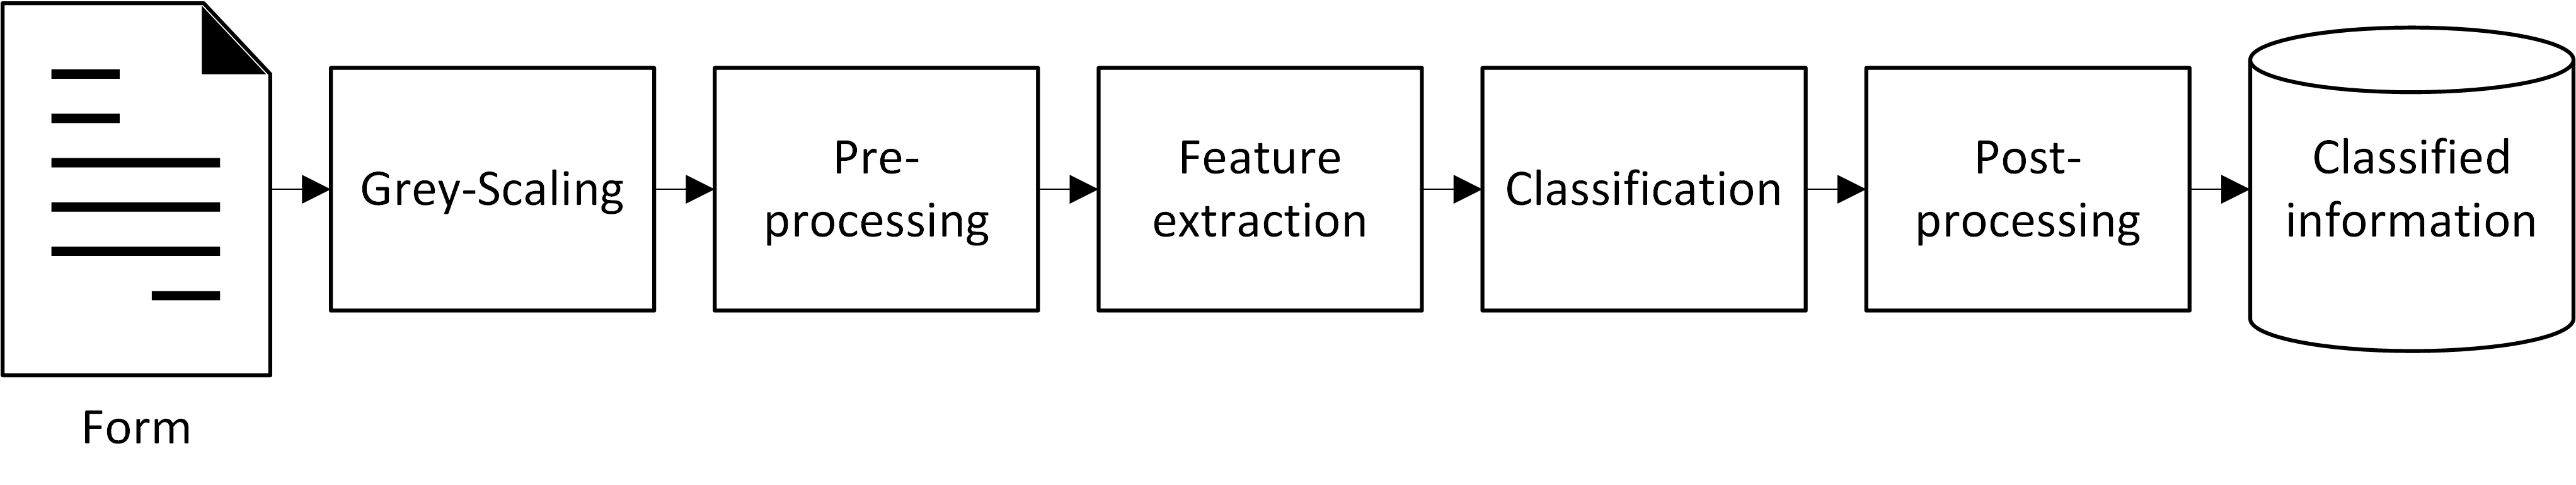
\includegraphics[width=100mm]{Images/OCR/Steps_Of_OCR.jpg}
\caption{Steps of OCR \label{ocrSteps}}
\end{figure}

The whole process of OCR is part of research since decades and several papers, dissertations and books have been published on the matter. Developing our own OCR algorithm would not only exceed the size of this master thesis, but also most likely retrieve less successful results than already developed and improved algorithms. Instead, this chapter will introduce several available OCR algorithms and compare open source solutions to find the best fit for our need.

\section{Currently available OCR algorithms}
\label{sec3.1}

OCR has been of interest for companies over many years. Hence we expect several possible solutions we could choose. As the amount of solutions can easily be very high we want to reduce the presented solutions to a maximum amount of 10.

Each description of a solution will contain information about the license used, the supported operating systems, programming languages used as well as if there is a software development kit. Also general information about the company will be given, the currently released version of the solution and the release date and, if existent, the number of languages supported.

\subsection{ABBYY Fine Reader}
\label{sec3.1.1}

ABBYY Fine Reader is a proprietary solution from the identically named company ABBYY founded in 1989. It is usable for all three operating systems, whereby linux-distributions are only supported as a command-line-interface. ABBYY supports a SDK for all three operating systems. Although it is written in C/C++ there exists a wrapper for java development for Linux and Windows\cite{abbyy16}. 

The SDK is currently in Version 11, it supports 185 languages, the latest update was on 03.10.2016.

\subsection{Anyline SDK}
\label{sec3.1.2}

Anyline is an Austrian company founded in 2013 who aim at OCR solutions for mobile systems. They offer their SDK as a free license for non-commercial use. However, as they are focused on mobile systems, they do not explicitly support Windows-Desktop, Linux or MacOS.

It can be developed with Java and Objective-C as well as Swift, C\# and Javascript. The current version of the SDK is 3.8.1 and has been released on 13.01.2017.

Currently supported are two languages: English and German.

\subsection{Asprise OCR}
\label{sec3.1.3}
Asprise has been founded in 1998 in Singapure. The company offers OCR SDKs in various programming languages (Java, C\#, VB.NET, Python, C/C++ and Delphi Pascal). The SDKs are under loyalty-free license and therefore proprietary. More than 20 languages are supported, English and German are included.
The SDK supports Windows, MacOS and Linux, whereby support of multiple operating systems at once increases the price.

\subsection{GOCR}
\label{sec3.1.4}
GOCR is an OCR application started by Joerg Schulenburg in 2000. The program is developed under the GNU Public License.\footnote{The project can be found here: http://jocr.sourceforge.net/, last visited on 06.03.2016}

The latest version is 0.5 and has been released in March 2013. It is working under Windows, Linux and MacOS. The code is written in C, but is not known if there is a SDK which enables usage of the application inside another application. The number of supported languages is also unkown.

\subsection{LEADTOOLS}
\label{sec3.1.5}
Leadtools is an American company founded in 1990 and offers various products in the range of document and image processing. 

The Leadtools OCR Engine can be used as an SDK and integrated in another application. Development with the SDK is possible with C\# and VB as well as C/C++ and Java (and some others). The engine supports more than 40 languages, containing German and can be used on Windows, Linux and MacOS. 

The current version of the SDK is 19 and has been released in December 2014.

\subsection{MathOCR}
\label{sec3.1.6}
MathOCR is a document recognition system written in Java with focus on formulas. The MathOCR project started in March 2014 and is based on the GNU General Public Liense.\footnote{The source code can be found here: https://sourceforge.net/projects/mathocr/, last visited on 06.03.2017}

The current version of the application is 0.0.3, which was released in May 2015 and is therefore still in a pre-alpha status. It can be used on Windows, Linux and MacOS. The amount of supported languages is not stated on the project page.

\subsection{OCROpus}
\label{sec3.1.7}
The OCRopus Open Source OCR System is an open source system developed and maintained by the German Research Laboratory for Artificial Intelligence under guidance by Thomas M. Breuel\footnote{The source code can be found here: https://github.com/tmbdev/ocropy, last visited on 06.03.2017}. It is licensed under the Apache 2.0 License. It was first published in 2008 \cite{Breuel08}.

The command-line application is written in Python and C++ and only supports Linux as Operating System. It currently uses the Tesseract as a text line recognizer but will be replace it in the future. 

The current stable version is 1.0 and has been released in November 2014. The amount of supported languages is unkown, whereby it is able to work with latin-based languages.

\label{OCRad}
\subsection{OCRad}
OCRad is a free OCR application under the GNU Public License and part of the GNU project \footnote{The project can be found here: https://www.gnu.org/software/ocrad/, last visited on 06.03.2017}. Antonio Diaz Diaz developed the application since 2003.

The current version is 0.25 and has been released in April 2015. It comes as a stand-alone console application but can also be used in the background by other applications.

\label{OmniPage}
\subsection{OmniPage Capture SDK}
The Nuance Communication Inc. offers an OCR tool called OmniPage Capture SDK, which enables document processing on Windows, Linux and MacOS. Depending on the underlying operating system it supports C/C++, Objective-C or C\# and VB.NET.

The current version is 20 and has been released in 2016. It supports over 120 languages (German included).

\label{Tesseract}
\subsection{Tesseract}
The Tesseract OCR Engine historically was an early project developed by Hewlett Packard between 1984 and 1994. In 2005, it was put on an open source license. It is currently maintained by Google under the Apache 2.0 license \cite{smith07}.

Tesseract is originally written in C/C++ and can be used on Windows, MacOS and Linux\footnote{The source code for tesseract can be found here: https://github.com/tesseract-ocr, last visited on 06.03.2017}. There also exists a wrapper which allows development in Java, the open source project Tess4J\footnote{The wrapper can be found on: http://tess4j.sourceforge.net/, last visited on 06.03.2017}.

The current stable version of the Tesseract is 3.04.01 and has been released in February 2016. It supports over 100 languages (including German). 

\label{OCRComparison}
\section{Comparison between open source algorithms}
While several companies exist that offer good OCR libraries and SDKs, we have to stick to free software, since we are not able to afford a proprietary license. In a later state of the application, it could be possible to switch to a proprietary solution in order to increase our OCR efficiency. Until then, we will decide for the best fitting open source algorithm library and improve our efficiency by preprocessing the forms ourselves. This is explained in Chapter 4, Module 1.

Upon the 10 presented solutions, only 5 are free for use. These are: GOCR, Tesseract, OCROpus, MathOCR and OCRad.

The following table shows the named solutions and shows their differences regarding their version, the latest release date, the supported programming languages and operating systems as well as the license they are put on:
% Please add the following required packages to your document preamble:
% \usepackage{graphicx}
% \usepackage[table,xcdraw]{xcolor}
% If you use beamer only pass "xcolor=table" option, i.e. \documentclass[xcolor=table]{beamer}
\begin{table}[!htb]
\centering
\resizebox{\textwidth}{!}{%
\begin{tabular}{lccccc}
\hline
Application                                                               & \textbf{GOCR}                                                                           & \textbf{Tesseract}                                                                           & \textbf{OCROpus}                                                               & \textbf{MathOCR}                                                                        & \textbf{OCRad}                                                                          \\ \hline
Version                                                                   &0.5                                                             & 3.04.01                                                              & 1.0                                                    & 0.0.3                                                           & 0.25                                                            \\ \hline
Release Date                                                              & 03.2013                                                         & 02.2016                                                              & 11.2014                                                & 05.2015                                                         & 04.2015                                                         \\ \hline
\begin{tabular}[c]{@{}l@{}}Supported Programming\\ Languages\end{tabular} & C                                                               & \begin{tabular}[c]{@{}c@{}}C/C++, \\ Java (with Tess4J)\end{tabular} & \begin{tabular}[c]{@{}c@{}}C++, \\ Python\end{tabular} & Java                                                            & C++                                                             \\ \hline
\begin{tabular}[c]{@{}l@{}}Supported Operating\\ Systems\end{tabular}     & \begin{tabular}[c]{@{}c@{}}Windows, Linux,\\ MacOS\end{tabular} & \begin{tabular}[c]{@{}c@{}}Windows, Linux,\\ MacOS\end{tabular}      & Linux                                                  & \begin{tabular}[c]{@{}c@{}}Windows, Linux,\\ MacOS\end{tabular} & \begin{tabular}[c]{@{}c@{}}Windows, Linux,\\ MacOS\end{tabular} \\ \hline
License                                                                   & \begin{tabular}[c]{@{}c@{}}GNU Public \\ License\end{tabular}   & Apache 2.0                                                           & Apache 2.0                                             & \begin{tabular}[c]{@{}c@{}}GNU Public \\ License\end{tabular}   & \begin{tabular}[c]{@{}c@{}}GNU Public \\ License\end{tabular}   \\ \hline
\end{tabular}%
}
\caption{Comparison between different OCR engines}
\label{ocrEngineComparison}
\end{table}

MathOCR is a relatively young application and therefore in a pre-alpha state. OCRad and GOCR are one step closer to the first major release. OCROpus has reached that state on November 2014. Tesseract is already on Version 3.04 and has recently released an alpha version of 4.0.

While Tesseract, OCROpus and OCRad are supporting C++, GOCR is only working with C whereas MathOCR is only Java. Tesseract is supporting C and Java as well (while using Tess4J as a wrapper). OCROpus instead is working with Python, too.

All solutions support Windows, Linux and MacOS except OCROpus, which is only working on Linux.

While GOCR, MathOCR and OCRad are licensed under the GNU Public License, Tesseract and OCROpus are licensed under the Apache 2.0 License. The difference between those two is mainly the following: Applications that are developed under usage of another program under the GNU Public License have to be licensed under the GNU Public License as well. The Apache 2.0 License allows usage of other application and enables free choice of licensing, but requires the mentioning of the underlying use of an Apache 2.0 licensed application.


\label{OCRDecision}
\section{Decision finding and explanation}
In the beginning of this thesis, it was defined that the application should work on a Linux based operating system and be written in Java. While all presented solutions support Linux as an Operating System, not all of them work with Java as a programming language. In addition to that, OCROpus only supports Linux, which is fine for the current focus of the application, but could be of an issue later on if it should be ported to another operating system.

MathOCR is in a pre-alpha state which makes it difficult to use due to several missing functionalities and persistent bugs in the code. As it is mostly focused on mathematical equations and formulas, we will not consider MathOCR any longer, even though it supports Java as a programming language. 

As explained in section 3.2, the GNU Public License requires our application to be licensed under the GNU Public License as well if we use another code which is licensed under this license. Therefore, the Apache 2.0 license is considered better, as it allows us to decide about the license for ourselves.

In the interest of the application, we want to use solutions that are up-to-date and are still under development. Therefore, the latest release date gives us insights about the activity on a project. Since a lot of open source projects suffer from missing developers, we expect longer development cycles. But the last version of GOCR has been released around 4 years ago. Hence we consider GOCR as not up-to-date anymore.

The following table shows the solutions again, but with underlying colors regarding their ability to fit to our problem. Green is used as a best fit, whereas red significates a major problem. Yellow shows that this attribute is not as good as others but no kick-out criterion. 

% Please add the following required packages to your document preamble:
% \usepackage{graphicx}
% \usepackage[table,xcdraw]{xcolor}
% If you use beamer only pass "xcolor=table" option, i.e. \documentclass[xcolor=table]{beamer}
\begin{table}[!htb]
\centering
\resizebox{\textwidth}{!}{%
\begin{tabular}{lccccc}
\hline
Application                                                               & \textbf{GOCR}                                                                           & \textbf{Tesseract}                                                                           & \textbf{OCROpus}                                                               & \textbf{MathOCR}                                                                        & \textbf{OCRad}                                                                          \\ \hline
Version                                                                   & \cellcolor[HTML]{FFFE65}0.5                                                             & \cellcolor[HTML]{34FF34}3.04.01                                                              & \cellcolor[HTML]{34FF34}1.0                                                    & \cellcolor[HTML]{FE0000}0.0.3                                                           & \cellcolor[HTML]{FFFE65}0.25                                                            \\ \hline
Release Date                                                              & \cellcolor[HTML]{FE0000}03.2013                                                         & \cellcolor[HTML]{34FF34}02.2016                                                              & \cellcolor[HTML]{FFFE65}11.2014                                                & \cellcolor[HTML]{34FF34}05.2015                                                         & \cellcolor[HTML]{34FF34}04.2015                                                         \\ \hline
\begin{tabular}[c]{@{}l@{}}Supported Programming\\ Languages\end{tabular} & \cellcolor[HTML]{FE0000}C                                                               & \cellcolor[HTML]{34FF34}\begin{tabular}[c]{@{}c@{}}C/C++, \\ Java (with Tess4J)\end{tabular} & \cellcolor[HTML]{FE0000}\begin{tabular}[c]{@{}c@{}}C++, \\ Python\end{tabular} & \cellcolor[HTML]{34FF34}Java                                                            & \cellcolor[HTML]{FE0000}C++                                                             \\ \hline
\begin{tabular}[c]{@{}l@{}}Supported Operating\\ Systems\end{tabular}     & \cellcolor[HTML]{34FF34}\begin{tabular}[c]{@{}c@{}}Windows, Linux,\\ MacOS\end{tabular} & \cellcolor[HTML]{34FF34}\begin{tabular}[c]{@{}c@{}}Windows, Linux,\\ MacOS\end{tabular}      & \cellcolor[HTML]{FFFE65}Linux                                                  & \cellcolor[HTML]{34FF34}\begin{tabular}[c]{@{}c@{}}Windows, Linux,\\ MacOS\end{tabular} & \cellcolor[HTML]{34FF34}\begin{tabular}[c]{@{}c@{}}Windows, Linux,\\ MacOS\end{tabular} \\ \hline
License                                                                   & \cellcolor[HTML]{FFFE65}\begin{tabular}[c]{@{}c@{}}GNU Public \\ License\end{tabular}   & \cellcolor[HTML]{34FF34}Apache 2.0                                                           & \cellcolor[HTML]{34FF34}Apache 2.0                                             & \cellcolor[HTML]{FFFE65}\begin{tabular}[c]{@{}c@{}}GNU Public \\ License\end{tabular}   & \cellcolor[HTML]{FFFE65}\begin{tabular}[c]{@{}c@{}}GNU Public \\ License\end{tabular}   \\ \hline
\end{tabular}%
}
\caption{Advantages and disadvantages of different OCR engines}
\label{ocrEngineRating}
\end{table}


As shown in the table, MathOCR will not fit our needs as it is a pre-alpha version. GOCR is outdated and also supports only C as a programming language. OCROpus and OCRad only support C++ (and in the case of OCROpus Python). In addition to that, OCROpus could be of a problem when porting the application to other operating systems whereas OCRad is licensed under the GNU Public License. 

Hence the Tesseract seems to be the best fit for our application. It is consistently updated and improved and by the history of it, the application itself has grown mature. The possibility to work with Tess4J enables the usage of it with Java. Multiple operating systems are supported and the Apache 2.0 license enables us to decide for ourselves under which license we will put the application.

   % (\chapter{OCR})
\cleardoublepage
%%%%%%%%%%%%%%%%%%%%%%%%%%%%%%%%%%%%%%%%%%%%%%%%%%%%%%%%%%%%%%%%%%%%%%%%%%%%%%%
%
% Machine Learning
% 
%%%%%%%%%%%%%%%%%%%%%%%%%%%%%%%%%%%%%%%%%%%%%%%%%%%%%%%%%%%%%%%%%%%%%%%%%%%%%%%
\chapter{Machine Learning}
\label{cha4}

The field of Machine Learning contains concepts how computers can obtain information without explicitly programming this kind of information retrieval. These concepts of ''Learning'' can be divided in three main categories: Supervised learning, Unsupervised learning and Reinforcement Learning.

Supervised learning always deals with a user that ''feeds'' input to the program as well as desired output. The program should recognize patterns that lead from the given input parameters to the desired output.
Unsupervised learning instead, is an approach where the program does have an input and needs to find a structure in those data. The finding of some pattern can be the goal of the program itself.

Using reinforcement learning, every output of the program is being valued by the user again. Output that has been found correctly will be strengthened, whereas incorrect values will act repulsive on the algorithm. After multiple iterations of this process, the program can find the best answer (but not always the correct answer) using the attracting and repulsive values.

Our goal is to use one machine learning technique in order to improve the outcome of our application. One major objective that can be addressed with Machine Learning is the relation between accounting record positions and how they are assigned to all the accounts that are important for this position.
We identify two major problems regarding this classification:
\begin{enumerate}
         \item What does a position represent?
         \item Which accounts should be assigned to this position?
\end{enumerate}
As we are processing an invoice, we will retrieve a position as a String. An accountant would be able to identify the position (which means a semantic identification of the object) and assign it to the accounts that are important in this matter. But, as there is no concrete rule which position belongs to which accounts, every company can apply this position to different accounts.

For instance, the maintenance of a car in the car pool of a company could be booked as car costs, or (if the company defines it more specifically) as maintenance, car parts and worker time.
Hence we need an algorithm that is capable of the following:
\begin{enumerate}
		\item Assign involved accounts depending on the user (-> allow different account structure)
		\item Learn relationships between a string and a set of accounts
\end{enumerate}
While the algorithm should be able to deal with those problems, we will have another problem to deal with: OCR errors (e.g. ''CAB'' instead of ''CAR'')\footnote{We used uppercase letters here to make the possibility of OCR errors between those two words more easily understandable.}  and similar words (e.g. plural words such as ''apples'' instead of ''apple''). 

Keeping those constraints in mind, we can start thinking about a Machine Learning technique that satisfies our goal or at least helps us to reach it.
To narrow our search, we also have to think about automation. As this application should be able to reduce the time an accountant needs to process an invoice, we want to make this process as automatically as possible. Using a supervised machine learning method would lead to an application, that requires to validate each invoice every time. Hence supervised machine learning algorithms will not be considered here.

\section{An abstract approach on accounting records}
\label{sec4.1}

Before we can compare different Machine Learning algorithms we have to think about the model that is used. On one hand, there is the position value which can be seen as a single String. On the other hand, we have 1195 Accounts (as proposed in the SK03 account system) that can be involved in this accounting process. Between those accounts, we also have to divide between accounts for debit and credit.

Evaluating each account per position would need two iterations: First if the account is relevant for this string and second if it is involved as a credit or debit account.
We come up with a different approach. As we see the position abstract as a string, we see the combination of accounts as a combined structure. This way we do not only reduce the iterations to one, but also enable a 1:1 relation.

For instance, given two accounts a1 and a2 we would have two possible structures: s1: {a1|a2} and s2: {a2|a1}\footnote{Each structure will be written the following way: The curly braces mark beginning and end of the structure, the pipe divides between credit and debit accounts.}. One time a1 is related to the credit side, one time to the debit side and vice-versa for a2. Given a position p1 there are now two possible structures we can assign p1 to.

The downside of this mapping from 1:N to 1:1 relations is the increasing number of possible solutions. But the advantage of it is the flexibility to assign a position to a known structure again after the user has defined how they want to it to be accounted.

\section{Possible machine learning algorithms}
\label{sec4.2}
We now know about how our model looks like. We also need an accountant initially to define how the position should be accounted. After these information have been given, the algorithm is able to assign a similar position to the same structure of debit and credit accounts. This means that we will look for an algorithm in the field of supervised learning.

There are several well-known algorithms in this field. For instance, Artificial Neural Networks (ANN), the K-Nearest-Neighbour Algorithm (KNN) or Decision Trees. To select the appropriate algorithm for our problem, we will be using a randomly generated trainingset consisting of a combination between 30 positions and 9 different structures in 1920 cases. We will evaluate the performance and accuracy of some of these algorithms to find the one that suits the most by using a testset of 2000 positions to be tested. To do so, we will be using an open-source software (RapidMiner Studio) that enables us to switch between those algorithms and evaluate the accuracy before implementing them.

The following table shows the algorithms and the accuracy as well as the time needed to evaluate the result:

% Please add the following required packages to your document preamble:
% \usepackage{booktabs}
% \usepackage{graphicx}
\begin{table}[!htb]
\centering
\scalebox{0.7}{
\begin{tabular}{@{}lcc@{}}
\toprule
Algorithm & \textbf{Accuracy} & \textbf{Duration} \\ \midrule
K-Nearest-Neighbour & 75,35\% & \textless1s \\ \midrule
Artifical Neural Network & 73,61\% & 30s \\ \midrule
Decision Trees & 72,92\% & \textless1s \\ \midrule
Na{\"i}ve Bayes & 72,92\% & \textless1s \\ \midrule
Random Forest & 55,03\% & \textless1s \\ \bottomrule
\end{tabular}%
}
\caption{Accuracy of different Machine Learning algorithms}
\label{mlAccuracy}
\end{table}

Except the Random Forest algorithm, there is not much of a difference between the algorithms. While Decision Trees and Na{\"i}ve Bayes result in the same accuracy, ANN are slightly more accurate. The disadvantage of this algorithm is its duration that increases exponentially by the amount of data. The data that we used resulted in a duration of around 30 seconds execution time. The K-Nearest Neighbour algorithm instead, while still as fast as the other algorithms, also results in a higher accuracy.

We will now introduce the remaining three algorithms and take a closer look on the results regarding the data set that we used. After that, we will decide which algorithm we want to use in our application.

\subsection{The K-Nearest-Neighbour algorithm}
\label{sec4.2.1}
The KNN algorithm tries to classify an object by using k neighbours of the object. Each of the k neighbours already have a class ci which enables the calculation of a likelihood value for the unclassified object.
If we would choose k = 1 then the object would be given the same class then the closest neighbour. But this can lead to wrong assumptions since only neighbour has been taken into account. Hence we would need to select a value for k > 1. The given accuracy from Table (TODO: REF) has been achieved with k = 5.
%TODO: MAKE Mathematical
When further investigating in the results provided by the algorithm we found something we did not expect. In our trainingsdata we defined a position p1 and two different structures s1 and s2. n times p1 has been classified to s1, and n times to s2. This means, p1 is equally distributed between those two classes. But the KNN algorithm resulted in a classification of s1 = 60\% and s2 = 40\%. This can be explained by the chosen value for k. As we defined k = 5, there were 5 neighbours, 2/5 that belonged to s2 and 3/5 that belonged to s1. And indeed, as we changed k to an even value (k = 6) we had the expected classification of 50\% for s1 and 50\% for s2.

This should be taken into consideration when using this algorithm. As we do not know how much different classes exist and the amount of classes can increase by the user assigning positions to new structures, we could have wrong classification values.

\subsection{Decision Trees}
\label{sec4.2.2}
Decision Trees are a simple and still effective way of classify an object to different classes. Usually the object that should be classified contains several attributes and each of them will be taken into consideration iteratively.

We want to explain the behaviour of decision trees on the following example: 
A telecommunication company had an increasing amount of customer loss recently. To find out the reasons behind that and to find out which actions to take to get new customers again, they build up a tree with the data they have of their customers. This decision tree can be seen in figure \ref{decisionTreeExample}.

\begin{figure}[ht!]
\centering
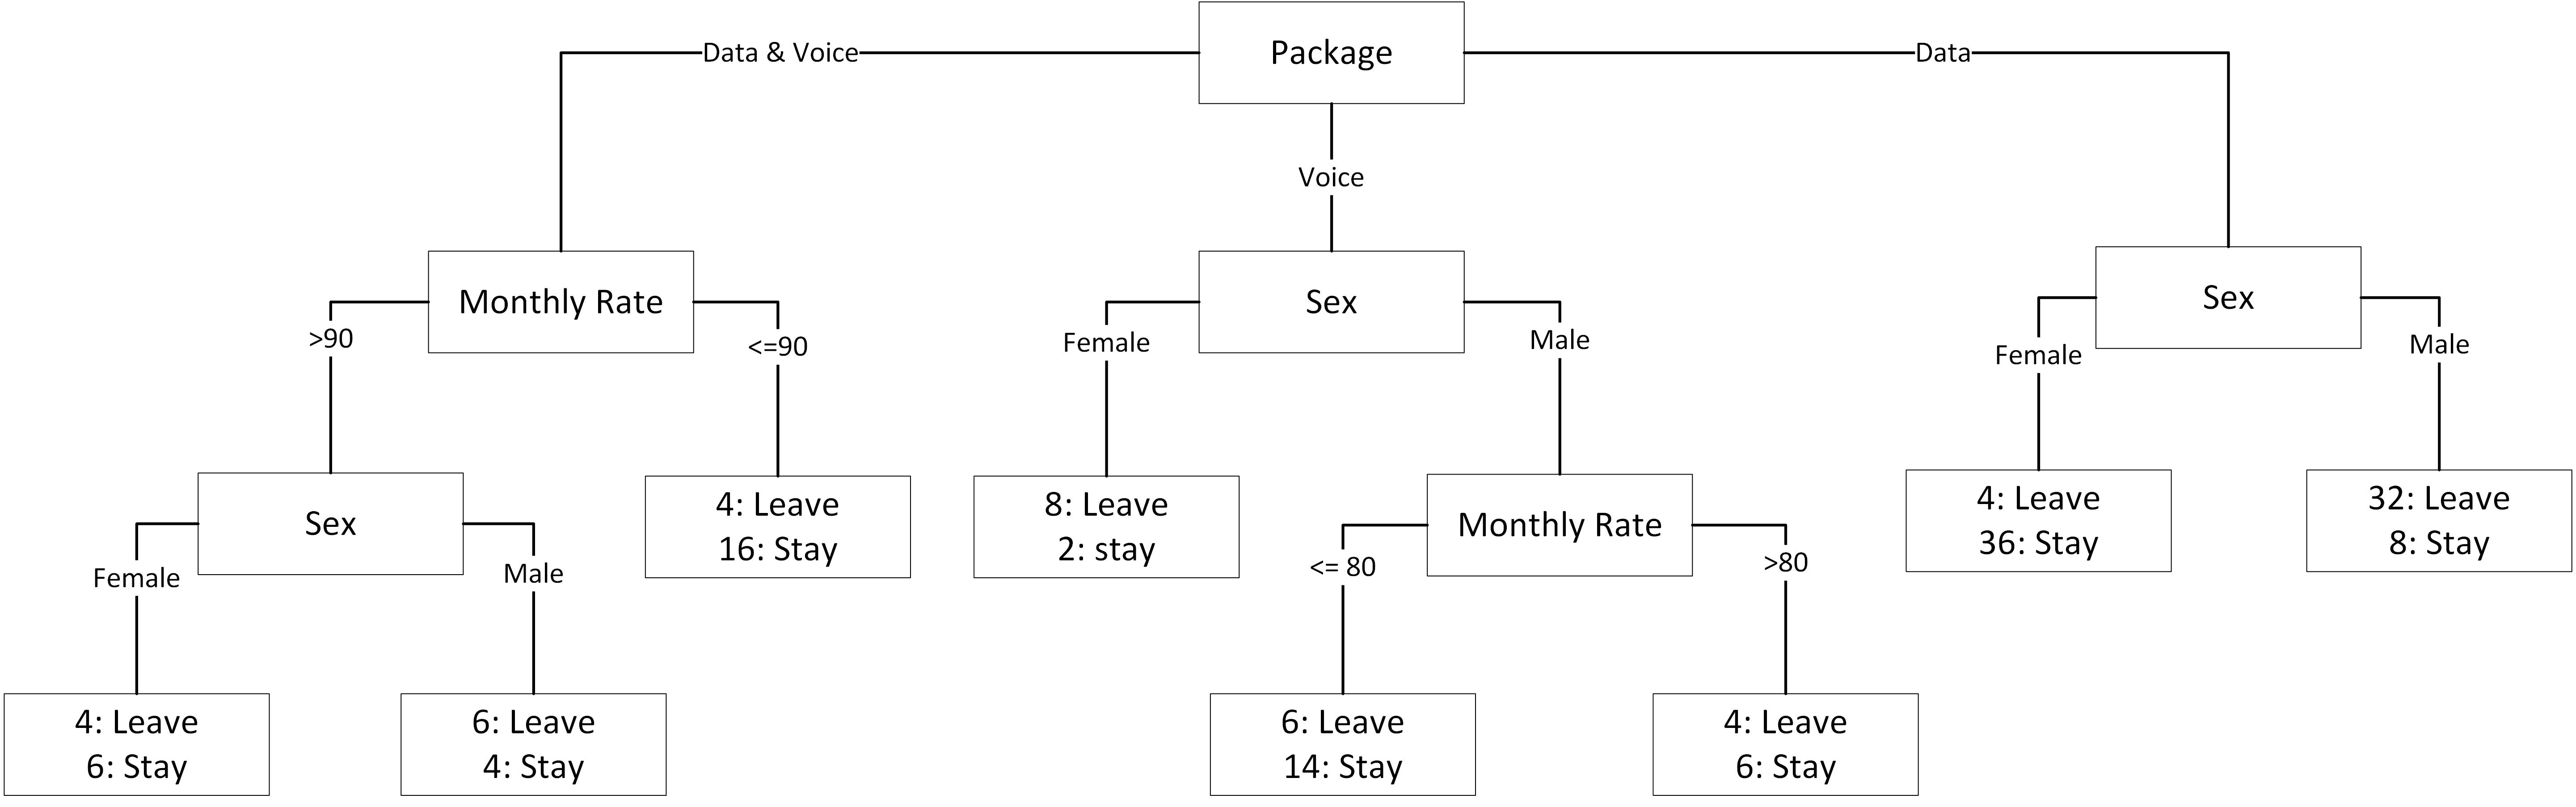
\includegraphics[width=\textwidth]{Images/ML/DecisionTreeExample.jpg}
\caption{Example of a decision tree \label{decisionTreeExample}}
\end{figure}

The companies offers three packages to their customers: Data, Voice and Data \& Voice. The data package has a high amount of male customers that left, whereas the most of the female customers stayed with the companies offer. The Voice package shows a difference between male customers that have been charged over 80 monetary units and the customers with a maximum of 80 monetary units.

Hence it is very likely that reducing the monthly rate for this package will result in a higher amount of customers staying with the offer of the company.

Using this decision tree, it is possible to split between objects even further, using different attributes. In our case, we only have the position as an attribute. If we would apply a decision tree on this problem, it would result in a tree with a depth of 1. This way the actual idea behind the decision tree is not used. The results would still be valid though.

\subsection{Na{\"i}ve Bayes}
\label{sec4.2.3}
Na{\"i}ve Bayes is a simple probabilistic classifier that calculates the probability that an object belongs to a class by taking each attribute of the object and comparing it with the probability of this attribute in the given class.

What this means for our case is the following: As we do not have any additional information on the position, the only attribute there is, is the string itself. This attribute is compared with the already classified positions. The result of this calculation will basically assign the position p to the class that has the most positions that are similar to p.

In addition to that, a way to improve the comparison is to use a numerical value that represents the similarity between the position p and another position that p is compared with. This can be done using the Levenshtein distance. The distance value represents the amount of changes needed to transform one position to the other. Using a relative value, we can make this result relative by the size of the position string:

\[
\frac {\text{Levenshtein distance}}{\text{Length of the position}}
\]

\section{Decision finding and explanation}
\label{sec4.3}

While we have excluded Random Forests due to the low accuracy as well as Artificial Neural Networks because of the long execution time from our list of choices, there are still three possible Machine Learning algorithms under consideration. We will now explain advantages and disadvantages of these algorithms and conclude this chapter by selecting one of these algorithms for our application.

All of the three algorithms are relatively easy to implement, the underlying concept is easily understandable (compared with some complex Machine Learning algorithms) and the resulting output of one of these algorithms is reasonable and traceable. 

As already mentioned in section \ref{sec4.2.2}, the concept of a decision tree would not fully used on our given problem. Decision trees are based on objects with multiple attributes and this can not be provided by our problem. Hence we will not use Decision Trees in our application.

Another problem has been mentioned in section \ref{sec4.2.1} before. When using the kNN classifier, the size of k has to be selected. Using a small k can lead to wrong classifications because of a bad classified neighbour. Choosing a high k could also lead to overfitting and would reduce the effectiveness of our method. But, since the amount of possible classes can (and will) increase over time, we would need to adjust k every time and therefore use another algorithm. Hence the usage of the kNN algorithm will not be considered anymore.
This means, that we will use a Na{\"i}ve Bayes approach in our application to classify positions to structures.    % (\chapter{Implementation})
\cleardoublepage
%%%%%%%%%%%%%%%%%%%%%%%%%%%%%%%%%%%%%%%%%%%%%%%%%%%%%%%%%%%%%%%%%%%%%%%%%%%%%%%
%
% Implementation of the application
% 
%%%%%%%%%%%%%%%%%%%%%%%%%%%%%%%%%%%%%%%%%%%%%%%%%%%%%%%%%%%%%%%%%%%%%%%%%%%%%%%
\chapter{Implementation of the application}
\label{cha5}

The application is structured by different packages. Each of them providing a specific benefit to the program as a whole. Before speaking about those modules, we will talk about the actual requirements of the application. After that, each module will be explained in detail and how it works. After that, the last section will deal with problems and possible solutions.

\section{Requirements definition}
\label{sec5.1}

Focus of this application is the possibility to automatically process forms and retrieve the data of the forms. Hence the application should be able to deal with several files and process them. But, since there is a big variety of forms and every company have different structures, retrieving all necessary information can fail. If this happens, a user has to review scanned documents that contain errors. If it doesn't fail, the data should be stored without the need of a review.

These requirements are visualized as a use case in figure \ref{totalApplicationCase}.

\begin{figure}[ht!]
\centering
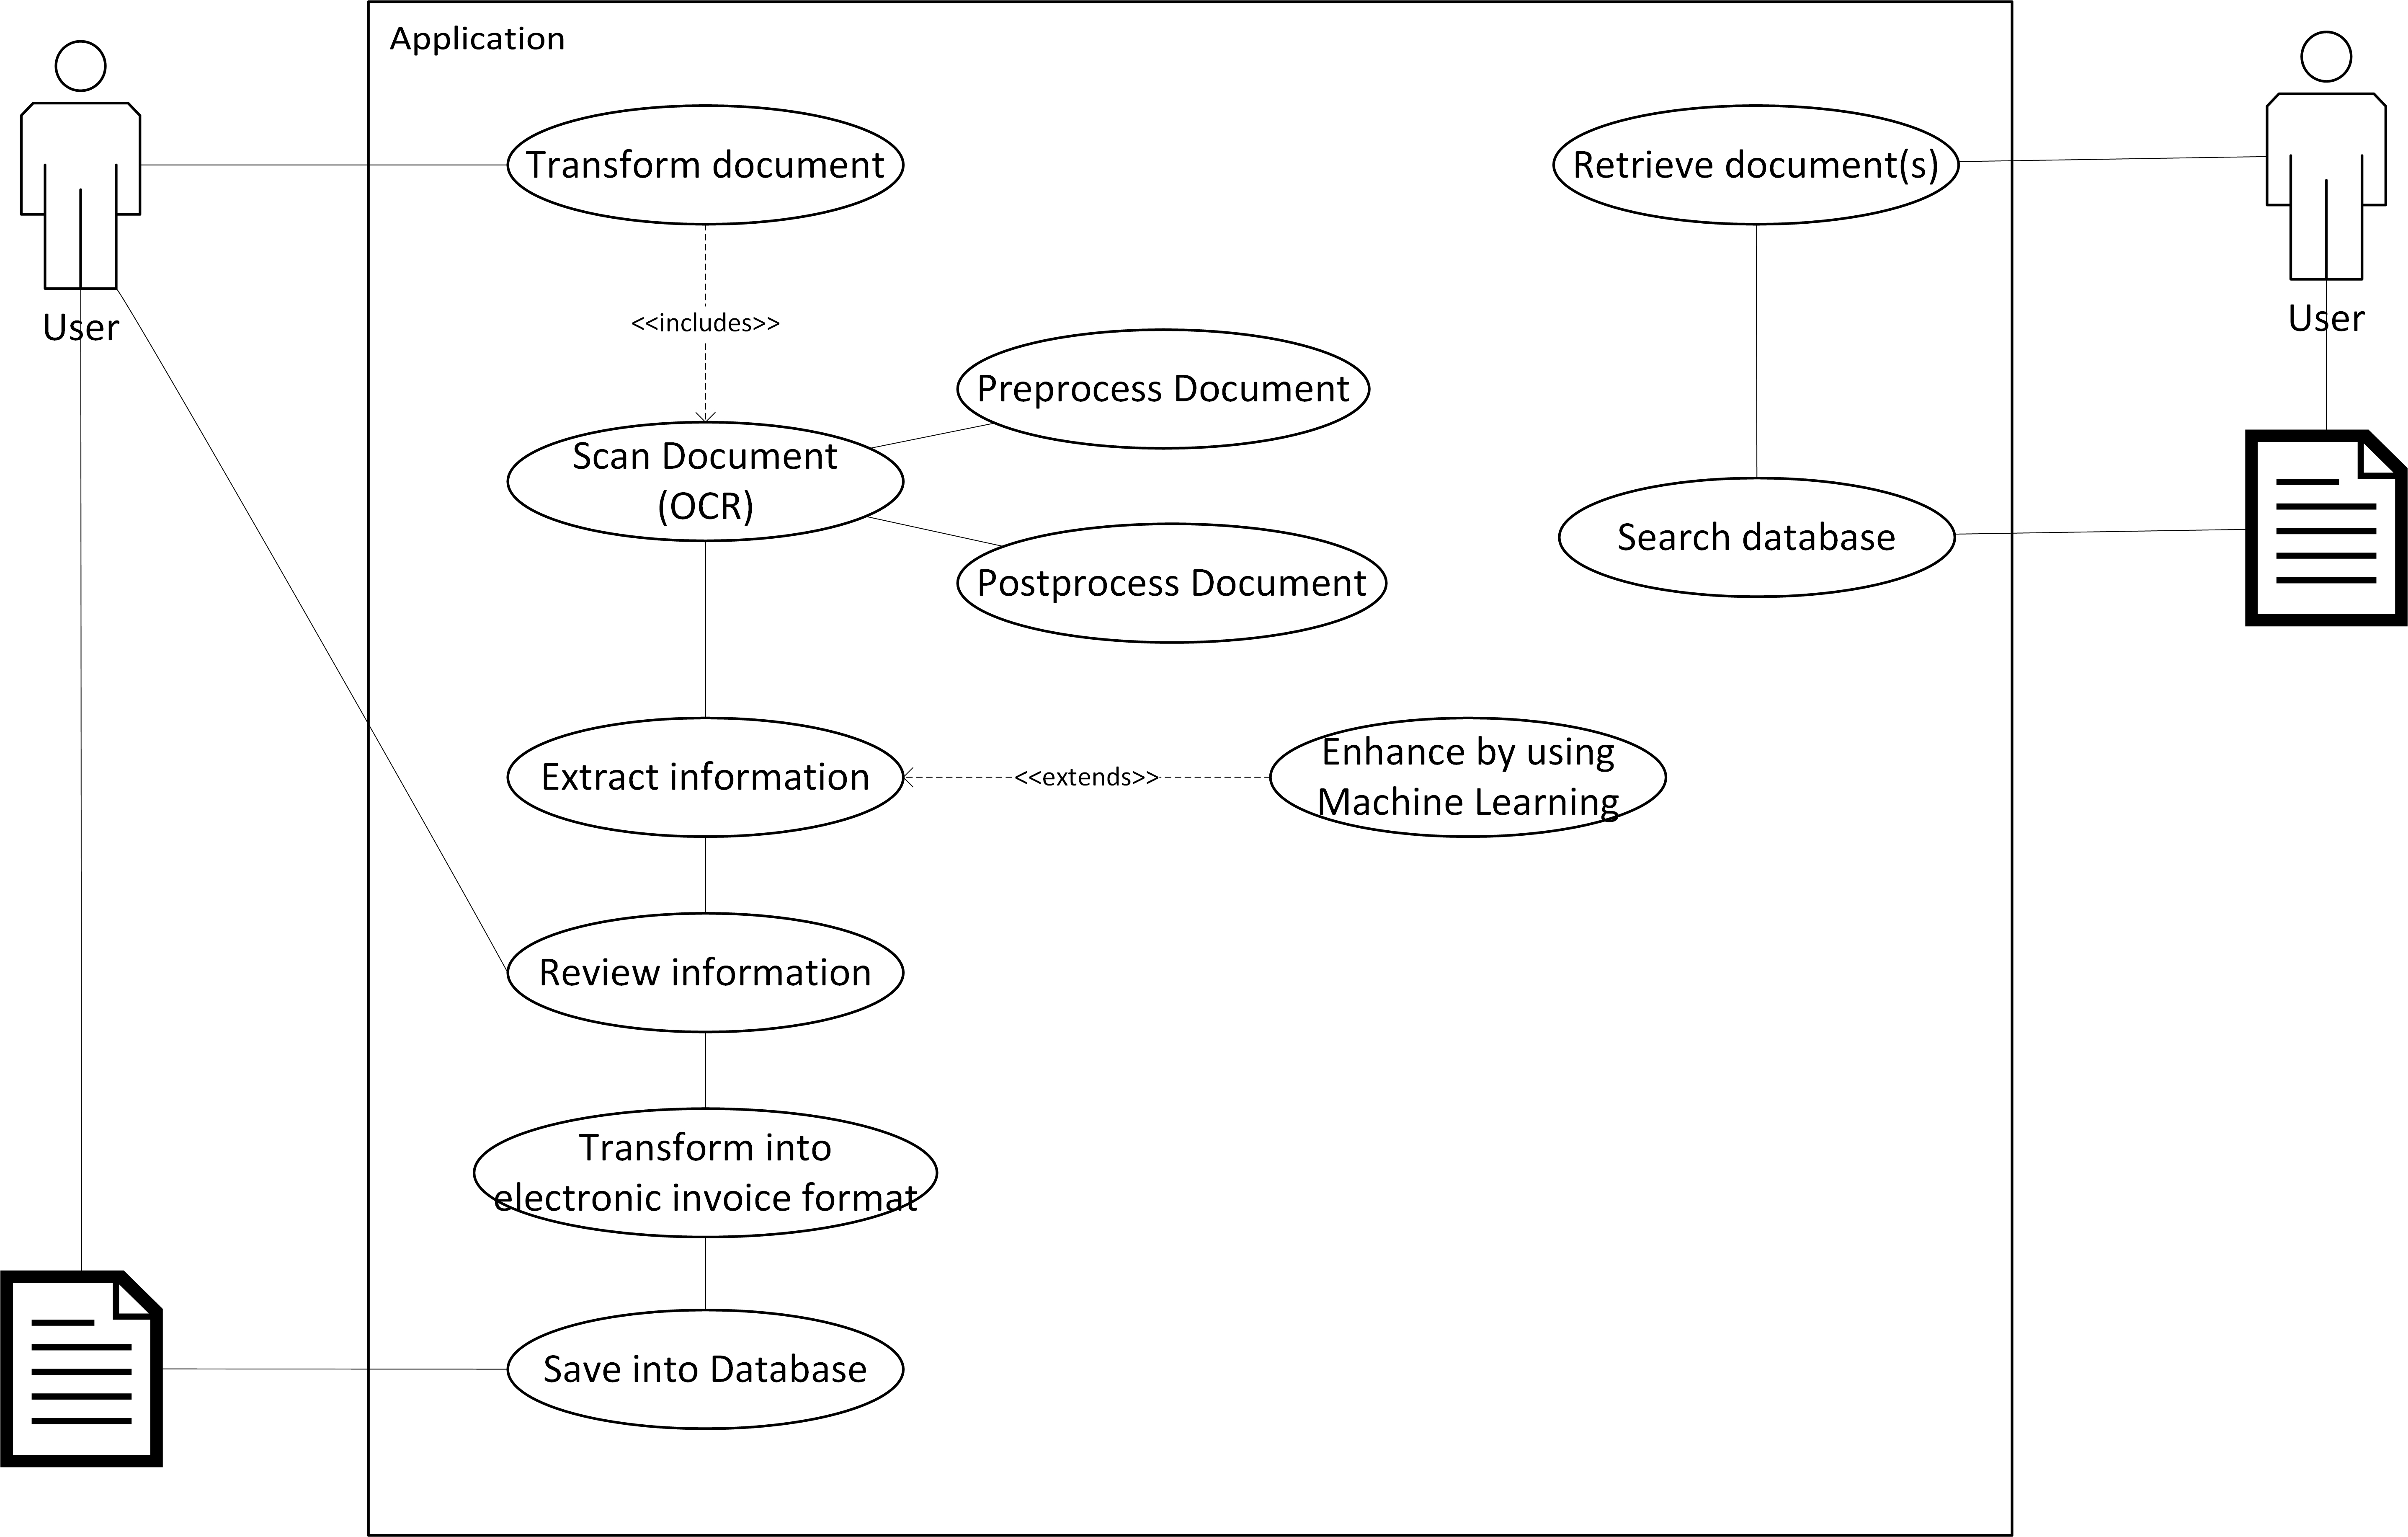
\includegraphics[width=\textwidth]{Images/UseCase/TotalApplicationCase.jpg}
\caption{Use case of the application \label{totalApplicationCase}}
\end{figure}

To improve the process of gathering data, a machine learning approach should be implement that facilitates retrieving data and to speed-up form processing over time.

Output of the application should be a storage of the processed forms, appended with electronic invoice information that is valid against the basic- or comfort-level of the ZugfErd-Invoice standard.

\section{Definition of modules}
\label{sec5.2}

Following the Separation of Concerns principle (SoC) we want to separate all logical parts of the application into different modules.
What the application will do is to take an invoice, read it (1), extract the information out of it (2), improve the information by using machine learning techniques (3) and eventually convert it to the ZugFerd-format (4). All these processes should be manageable for the user using a GUI (5).
Hence we will define five different modules:
\begin{enumerate}
	\item OCR: After the user has passed an document to the application, this module will process the document and read it using OCR techniques. Therefore, this module will be named \"OCR\".
	\item Extraction: This module will deal with the business logic regarding the retrieval of information from the processed document. Therefore, it will also give input and get output from the third module.
	\item ML: In this module we will implement methods to improve future information extraction.
	\item Transformation: Eventually, the extracted information and the processed document will be transformed into a new electronic invoice that is conform with the ZUGfERD-format.
	\item GUI: In order to facilitate the process of entering and retrieving invoices, another module will be used that deals with all sorts of user interaction. As this application will have an graphical user interface, we will call this module GUI.
\end{enumerate}

\section{Architectural concept}

The application is structured by different packages that each contribute to the application as a whole.
As shown in figure \ref{applicationUML}, there are 7 different packages. 

\begin{figure}[ht!]
\centering
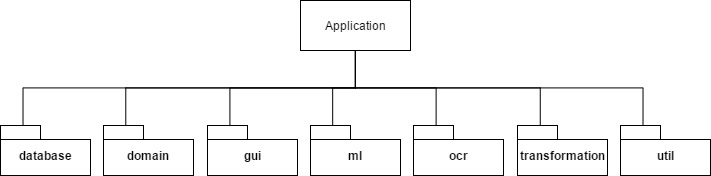
\includegraphics[width=\textwidth]{Images/UML/ApplicationUML.jpg}
\caption{Packages of the application \label{applicationUML}}
\end{figure}

In section \ref{sec5.2} we have already defined most of the packages before. However, we want to explain the other packages as well. While the modules OCR, ML, Transformation and GUI are present, the module Extraction is missing. The reason for that is that the actual extraction of information is a domain specific part of our application. Hence it can be found in the domain package. Figure \ref{domainUML} shows a detailed view of the domain package. This package again is structured by the subpackages 'bo', 'dao', 'helper' and 'service'.

\begin{figure}[ht!]
\centering
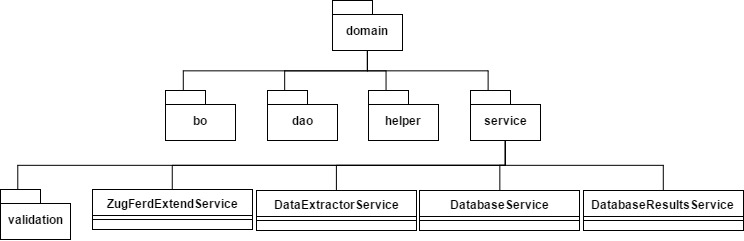
\includegraphics[width=\textwidth]{Images/UML/DomainUML.jpg}
\caption{The domain package in detail \label{domainUML}}
\end{figure}

'Service' contains the DataExtractorService class which is responsible for the actual extraction of invoice information. To do this, several other classes are called, some of them located in other packages (e.g. the utils package).

Besides the DataExtractorService class, there are other important classes. The ZugFerdExtendService class adds the valid ZugFerd invoice to the pdf document. The DatabaseService is responsible for saving the reviewed invoice documents (as the last part of the use case in \ref{totalApplicationCase}). When a user searches for invoice documents, the DatabaseResultsService is called that performs the actual request.

In addition to those classes, the package validation also contains classes to validate not only the mandatory invoice information, but also the accounting records.

The application will make use of an architectural design pattern, the Model-View-Controller (MVC) pattern.
This pattern separates the application in three parts: The model, that contains the data of a domain, the view, which presents the given data in a specific way to the user, and the controller, that is responsible for the communication between the other two. Figure \ref{MVCpattern} visualizes this behaviour.

\begin{figure}[ht!]
\centering
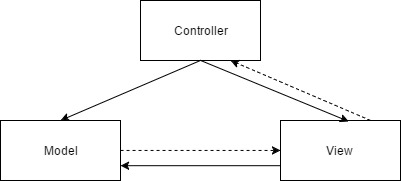
\includegraphics[width=100mm]{Images/UML/MVC.jpg}
\caption{The Model-View-Controller pattern \label{MVCpattern}}
\end{figure}

Using this architectural pattern, we are more flexible and can easily change views or models since these are only loosely coupled. Hence the graphical user interface will be steered by a controller which retrieves data from the database and shows it to the user using the javaFX framework and .fxml-Files (those represent the 'View' in the MVC pattern). Input and changes the user makes in the view will be transported by the controller to the model which is stored in the database again.

To access the database we will use classes for each business object. The package BO contains classes that represent a table. A data-access-object (DAO) will be used to retrieve data from the database. Note that these two packages are present in the domain package (see figure \ref{domainUML}).
This application will also make use of an object-relational mapping framework (Hibernate), which facilitates the conversation between table data and java objects.

\section{Module 1 - OCR}

The OCR module deals with the processing of the document. Therefore, we will use Googles Tesseract as described in chapter 3. In order to use it, we use Tess4J as a Java wrapper. TesseractWrapper.java is the class that initiates a tesseract instance. With initOcr() the tesseract instance is getting called. It returns a String as result. 

We set HOCR to true, which means that our output will not only be a String containing the processed words, but in a structured way. HOCR is a xml-structured document first proposed by \cite{Breuel07}. Using this output we are not only able to retrieve the processed words, but also their position in the document.

The package hocr contains necessary java classes to represent this document in an objective-oriented way. The string output of the TesseractWrapper class can be given to the constructor of the HocrDocument class, that completely parses the string and divides it into multiple HocrAreas, HocrParagraphs, HocrLines and HocrWords.
Before the actual step of processing the image, we want to improve its quality. Therefore, we use the ImagePreprocesser class. Any kind of document inserted will first converted to a BufferedImage. Then preprocess() can be called which executes multiple algorithms on the image:

\begin{lstlisting}[caption={Image preprocessing}]
public BufferedImage preprocess() {
    try {
        ...
        BufferedImage outputFile = this.resizeImage(image);
		...
        outputFile = this.adjustDPI(image);
		...
        outputFile = this.deSkewImage(image);
		...
        outputFile = this.greyScaleImage(image);
		...
        outputFile = this.deSpeckleImage(image);
		...
        return outputFile;
        } 
  	...
}
\end{lstlisting}

Most of those calculations are made using ImageMagick, a powerful open source library with several useful commands to apply on images. It is licensed under the Apache 2.0 license. In order to use it inside our application we are using IM4Java which is cited by ImageMagick itself\footnote{the citation can be found here: https://www.imagemagick.org/script/develop.php, last visited on 06.03.2017} and is licensed under the LGPL license.

\begin{figure}[htb!]
\centering
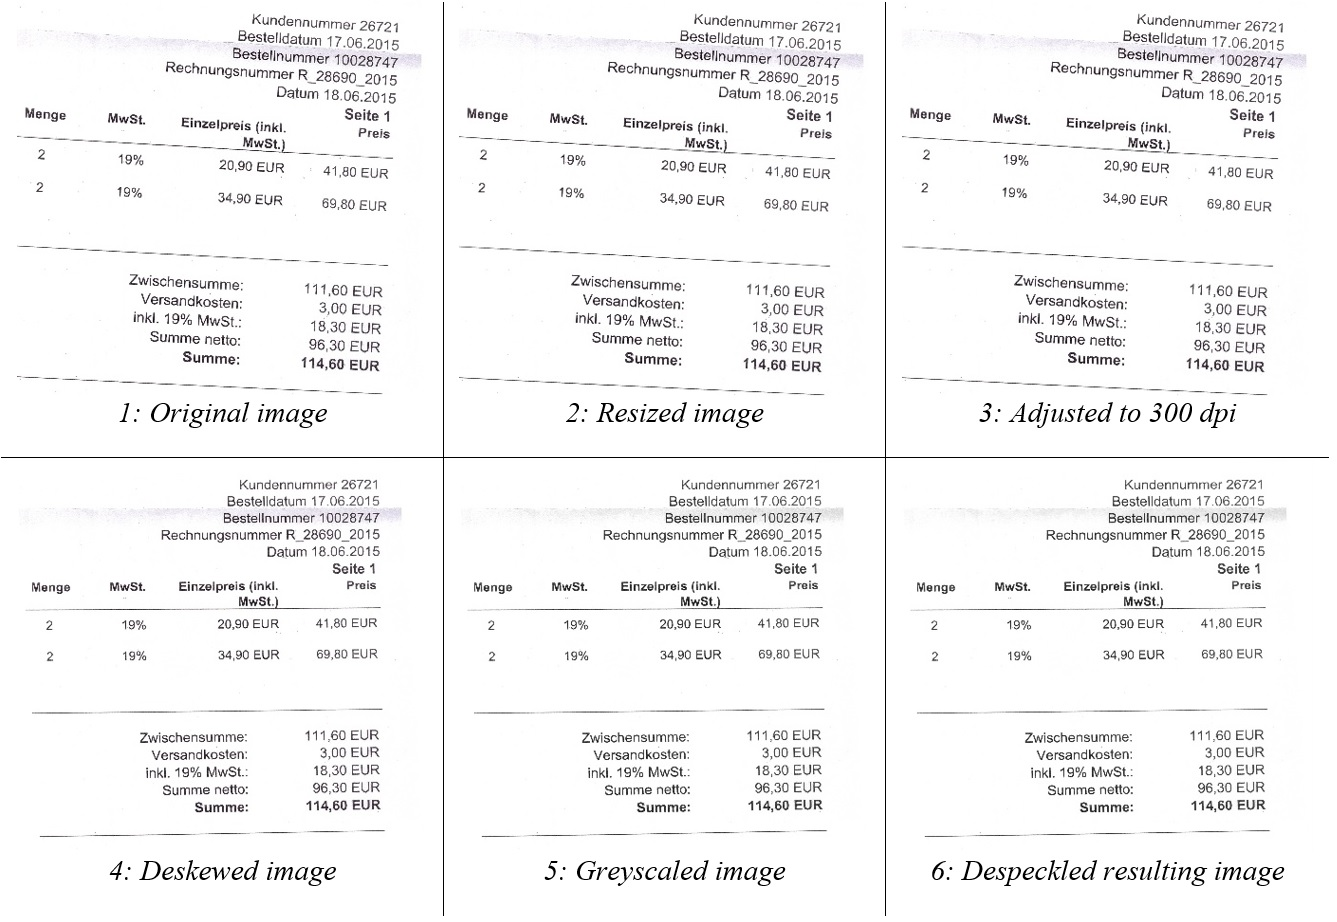
\includegraphics[width=\textwidth]{Images/OCR/PreprocessingSteps.jpg}
\caption{Preprocessing steps \label{preprocessingSteps}}
\end{figure}

The resulting changes in the image during the preprocessing steps are shown in figure \ref{preprocessingSteps}.
Especially the deskewing step and the greyscaling of the image can be seen very well.

In order to increase the performance of the application, we want to be able to perform the optical character recognition by using multiple instances of the tesseract at the same time. Hence we need to implement the Runnable interface provided by the JDK. 

Seen from the outside, the TesseractWrapper class is just the Tesseract instance itself. So we need a worker class that can be given to a new Thread. The TesseractWorker class implements this interface. When we start a new Thread using start(), the run()-method of this worker is called internally. Run initiates a new Tesseract instance and executes OCR with the given ocr file: 

\begin{lstlisting}[caption={Initiation of the OCR wrapper}]
/**
 * Executes tesseract ocr using a wrapper
 * The result can be obtained using the getResultIfFinished() method
 */
@Override
public void run() {
    TesseractWrapper wrapper = new TesseractWrapper();
    if (this.imgToScan == null) {
        this.result = wrapper.initOcr(this.fileToScan, runWithHocr);
    } else {
        this.result = wrapper.initOcr(this.imgToScan, runWithHocr);
    }
    Logger.getLogger(this.getClass()).log(Level.INFO, "Finished OCR");
}
\end{lstlisting}

Since we want to be able to support not only pdf documents, but also images, we have to differentiate between this two. Depending what type of document, we have to parse it differently in order to get a BufferedImage out of it.

After the OCR process took place, we have a HOCRDocument. It may be that some of the values are wrong, e.g. have a wrong but similar looking letter in it. This is not a problem as long as specific keywords are not affected. Recognizing such keywords in the document is crucial for the next steps. Hence we want to improve those values afterwards. 
The Postprocessor class targets this goal by going through the HOCRDocument:

\begin{lstlisting}[caption={Postprocessing the hocr document}]
        List<String> correctWords = this.readDictionaryValues();
        for (HocrPage page : this.documentToProcess.getPages()) {
            for (HocrElement area : page.getSubElements()) {
                for (HocrElement paragraph : area.getSubElements()) {
                    for (HocrElement line : paragraph.getSubElements()) {
                        for (int i = 0; i < line.getSubElements().size(); i++) {
                            HocrWord w = (HocrWord) line.getSubElements().get(i);
                            for (String dictWord : correctWords) {
                                // replace the word if the dictionary word is probably the right word
                                double confidenceRate = ConfigHelper.getConfidenceRate();
                                double distance = StringUtils.getLevenshteinDistance(w.getValue().toLowerCase().trim(), dictWord.toLowerCase().trim());
                                double comparison = distance / w.getValue().length();
                                if (comparison < confidenceRate) {
                                    w.setValue(dictWord);
                                    line.getSubElements().set(i, w);
                                    break;
                                }
                            }
                        }
                    }
                }
            }
        }
        return this.documentToProcess;
\end{lstlisting}

This is done using a dictionary of keywords. This dictionary is present as a file 'keywords.txt' and enables further improvements by the user (e.g. adding more keywords because of invoice documents in other languages).
The distance is calculated using the Levenshtein distance again. If the distance is small enough, the value of the HocrWord object is replaced by the keyword in the keywords.txt file.

Now that we have executed the OCR step and postprocessed the resulting values, the next module can go on in the complete process.

\section{Module 2 - Extraction}

The core class that extracts the information from the hocr document is the DataExtractorService class. As we also want to retrieve information as fast as possible, we want to run it on different threads, so that we can extract the invoice information part on one thread and the accounting records information on another. Hence this class needs to implement the Runnable interface. When instantiated, a flag is set if this thread should extract the former or the latter:

\begin{lstlisting}[caption={Beginning of the information extraction}]
@Override
public void run() {
    ...
    if (this.extractInvoice) {
        this.threadInvoice = this.extractInvoiceInformationFromHocr();
    } else {
        this.threadRecord = this.extractAccountingRecordInformation();
    }
}
\end{lstlisting}

We will now start explaining the extractInvoiceInformationFromHocr() method in detail before continuing with the explanation of the extractAccountingRecordInformatio() method.
As we built our invoice information extraction process on similar invoices of the same creditor, the extractInvoiceInformationFromHocr() method starts with a search for the creditor:

\begin{lstlisting}[caption={Call for creditor in the database}]
...
result.setCreditor(this.getLegalPersonFromDatabase(this.getHocrDoument(), true));
if (result.getCreditor() != null) {
    result = this.getCaseInformation(result);
} else {
    String invNo = this.findInvoiceNumber();
    result.setInvoiceNumber(invNo);
    result.setIssueDate(this.findIssueDate());
    result.setDebitor(this.getLegalPersonFromDatabase(this.getHocrDoument(), false));
}
...
\end{lstlisting}

If we are not able to find the creditor in the database (because there was no invoice of this creditor yet) we will continue by searching for necessary invoice information by hand. This will be covered after the case information retrieval.

If a creditor is found, we get the case information of the corresponding creditor. A DocumentCase consists of a creditor to which it belongs as well as a keyword which relates the DocumentCase to one of the following:
\begin{itemize}
	\item Document type: The DocumentCase contains information where to find a keyword that defines the document as an invoice, a proforma invoice or a credit note.
	\item Invoice number: The DocumentCase contains information where to find the corresponding invoice number of the invoice.
	\item Invoice date: The DocumentCase contains information where the invoice date is being placed on the document.
	\item Creditor: The DocumentCase contains information where the name of the creditor usually is. This is being used for new documents that are not classified yet in order to improve the recognition of creditors.
	\item Debitor: The DocumentCase contains information where the name of the debitor usually is.
\end{itemize}

Besides the keyword and the creditor, there is also the position stored where one of those keywords can be found, as well as the creation date of the DocumentCase, which is being used so that newer cases get a higher priority. This way we can react on changing designs for example when a company decides to restructure their invoice documents.

In addition to that, a case id clusters all DocumentCases that are created on one document. With five keywords at hand, a maximum of five DocumentCases should be related to one document.

A flag isCorrect is also existing but set to false in the beginning. After the user has reviewed missing information and wants to store the revised documents, the case is compared with the given information. If there are no changes, we expect the case to be correct. Hence at this time we set isCorrect to true.
The getCaseInformation() method first retrieves all cases from the found creditor. Then, it sorts them to the corresponding cases.

For each keyword the corresponding cases contain position information of older documents where the keyword has been found. With that position at hand, the current HOCR document is being searched for a value at that position. The method findInCase() deals with this process:

\begin{lstlisting}[caption={Search for information in the DocumentCase}]
private HocrElement findInCase(List<DocumentCase> cases) {
    for (DocumentCase docCase : cases) {
        if (docCase.getIsCorrect()) {
            String[] position = docCase.getPosition().split("\\+");
            // 0: startX, 1: startY, 2: endX, 3: endY
            int[] pos = new int[] {
				Integer.valueOf(position[0]), 
				Integer.valueOf(position[1]), 
				Integer.valueOf(position[2]), 
				Integer.valueOf(position[3])
			};

            HocrElement possibleArea = this.document.getPage(0).getByPosition(pos, 50);
            if (possibleArea != null) {
                HocrParagraph possibleParagraph = (HocrParagraph)  possibleArea.getByPosition(pos, 30);
                if (possibleParagraph != null) {
                    HocrLine possibleLine = (HocrLine) possibleParagraph.getByPosition(pos, 30);
                    if (possibleLine != null) {
                        HocrWord possibleWord = (HocrWord) possibleLine.getByPosition(pos, 10);
                        if (possibleWord != null) {
                            return possibleWord;
                        } else {
                            // refine to multiple words, pixel threshold only a few pixels since we are searching for word
                            possibleWord = possibleLine.getWordsByPosition(pos, 10);
                            return possibleWord;
                        }
                    }
                }
            }
        }
    }
    return null;
}
\end{lstlisting}

We are only using the cases that have the flag isCorrect set to true. Then we compare all HocrElements in the document with the stored position. But, as there could also be some small differences (e.g. because the scans are hand-made and the document has not been placed on the exact same position every time) we apply a threshold value. Every element that is more or less consistent with the given position will be returned. Eventually, we will a word that matches the position, or, if the position stored contained multiple words, a combination of words. Those are concatenated and returned. If any of those steps fail, the method will return null.

This is repeated for each keyword. A new DocumentCase is created and the position added. Every keyword that has not been found will result in missing DocumentCases. After that, the invoice filled with the retrieved information will be returned.

As mentioned before, if we are unable to find a creditor, then we proceed with the document manually. Which means we are looking for keywords such as ''Rechnungsnummer'' (invoice no.) or ''Rechnungsdatum'' (invoice date) which are usually followed by the corresponding value. This is a fallback practice and will yield more errors due to missing position information. An invoice object with the found values will be returned all the same.

The extractAccountingRecordInformation() method deals with the problem of information retrieval with a different approach: It uses the extracted table information if a table has been found (TODO: Include in text). If not, the HocrDocument is searched for keywords that are usually appear in invoice tables.

The detection of a table is done using another class, the HistogramMaker. 

If we find those information, we iterate over the following lines until we find table end information, such as ''Gesamtbetrag'' (total value), ''Lieferdatum'' (delivery date) and others. Both, the table header words as well as table end words are stored in two textfiles (tablecontents.txt and tableendings.txt) which allows the user to add more words to improve the accuracy.
Now, every line will be processed the following way:

\begin{lstlisting}[caption={Extraction of accounting record information},label={arExtraction}]
Record r = new Record();
String recordLine = this.removeFinancialInformationFromRecordLine(nextLine);
double value = this.getValueFromLine(nextLine);

Model m = service.getMostLikelyModel(recordLine); 
if (m == null) {
    r.setEntryText(nextLine);
} else {
    r.setEntryText(m.getPosition());
    r.setRecordAccounts(m.getAsAccountRecord(value));
    r.setProbability(m.getProbability());
}
records.add(r);
index++;
\end{lstlisting}

We first want to remove all those additional information from the position so that we are able to store / retrieve it if it comes again more precisely. This is done by the removeFinancialInformationFromRecordLine() method. After that, we also retrieve the total amount of the position by searching in the line again for the financial information, but this time searching for the last numeric value that is proceeded by ''EUR'' or ''\euro''.

After that, the machine learning module is called. What exactly happens there will be covered by the next section. We will retrieve a possible Model that applies to our position. We can assign the found value to every involved account as the Model also contains the percentual values of each account and add a probability value to the Record which will later presented to the user in order to facilitate his decision if the automatically made decision is correct or not.


\section{Module 3 - Machine Learning}

The Model object shown in listing \ref{arExtraction} is a combination of debit and credit accounts (stored as a map with the corresponding values), the position string and the probability value. The LearningService class is the core class of this module and is getting called using the getMostLikelyModel() function. What this method does is the following:

\begin{lstlisting}[caption={Search for the most likely model}]
 public Model getMostLikelyModel(String feature) {
        String replacedString = feature;
        NaiveBayesHelper helper = new NaiveBayesHelper();
        ModelReader reader = new ModelReader();
        ...
            helper.trainClassifier(reader.getModels());

            // replace string if it is equal with an existing value
            for (Model m : reader.getModels()) {
                if (m.positionEqualsWith(feature)) {
                    replacedString = m.getPosition();
                    break;
                }
            }
		...
\end{lstlisting}

In the first part, the NaiveBayesHelper is called, that trains the classifier with all models that are stored. Every time the user saves an invoice document, all the accounting records are transformed into this model and saved to a file. The ModelReader takes these information for the next classification and hands it to the NaiveBayesHelper that is training the classifier.


To use the naive bayes classifier, we make use of a small implementation by Philipp Nolte, licensed under the MIT license\footnote{See also: https://github.com/ptnplanet/Java-Naive-Bayes-Classifier (Retrieved March 5, 2017)}.

When the classifier has been trained by the existing data, we compare the position with the ones stored in the existing models. This is done by a call to the model with positionEqualsWith(), that not simply compares the string, but also calculates the levenshtein distance. This is shown in listing \ref{positionComparison}.

\begin{lstlisting}[caption={Comparison between positions},label={positionComparison}]
    boolean positionEqualsWith(String positionToCompare) {
        int levDistance = StringUtils.getLevenshteinDistance(this.getPosition(), positionToCompare);
        int length = this.getPosition().length();
        double distance = (double) levDistance / (double) length;
        if (distance < 1 - ConfigHelper.getConfidenceRate()) {
            return true;
        } else {
            return false;
        }
    }
\end{lstlisting}

In the second part, the classifier is called and should now start classify the position. What this classifier does is basically the same as explained in section \ref{sec4.2.3}. The classification object also contains a probability value. We want this probability higher than a user set confidence rate in order to use the model.

If  this is the case, the ModelReader will be called again to retrieve the found model. This model will also be now be used in the transformation process 

\begin{lstlisting}[caption={Classification of a position}]
        Classification<String, List<Account>> classification = helper.getClassifier().classify(Collections.singleton(replacedString));
        if (classification.getProbability() > ConfigHelper.getConfidenceRate()) {
            try {
                Model m = reader.getModelByStringAndAccounts(String.valueOf(classification.getFeatureset().toArray()[0]), classification.getCategory());
                m.setProbability(classification.getProbability());
                return m;
            } catch (IOException e) {
                e.printStackTrace();
                return null;
            }
        }
        return null;
    }
\end{lstlisting}

However, if the probability is below the confidence rate, or any other problem might occur, null will be returned. This way only the position value will be set and the user has to manually check this accounting record (as can be seen in listing \ref{arExtraction}).
    
\section{Module 4 - Transformation}

We have now extracted required basic information of the invoice as well as accounting records based on the positions in the invoice. Everything has been labelled by a confidence level in the application. All documents with a confidence level lower than previously defined by the user had to be reviewed by the user manually.
The final part of the use case is the transformation of those extracted information into the ZugFerd invoice format. Therefore, we need to order the given information in a predefined format and append it as xml-information to the invoice pdf.

We are using the Mustang project to generate the xml content for us. It is an open source project licensed under the Apache license version 2.0 and currently under version 1.3. This way, the amount of classes we need will be reduced to only one: The ZugFerdTransformator.java class.

Before giving an in-depth explanation about our implementation, we first want to explain how the ZugFerd-Format works.

\subsection{About the ZugFerd Scheme}

ZugFerd has been developed to close the gap between manually sent invoices in small companies and heavy electronic data interchange (EDI) between big companies. While EDI with its sub-standards can be a good solution for a big company, most of the small and medium sized companies can not make use of such a standard due to the overwhelming complexity that lies beyond this standard. But dealing with pdf documents manually is also a source of costs, errors and is time consuming.

ZugFerd stands in the middle between those two sides (TODO: ADD IMAGE). While documents can still be sent as a pdf, the underlying format enables automatic processing of the invoice. The extendibility with basic, comfort and extended levels enables also big companies to make use of this standard. This also improves the B2B relations between big and small companies.

Depending on the desired level of the ZugFerd format, more fields have to be filled out. But even the lowest level, the basic level, brings the possibility to provide additional information which would only be required on the comfort or extended level. But there are still some fields that even on the basic level are required. Those will be introduced now and explained shortly.
\begin{itemize}
	\item Document Context Parameter: This field describes which level will be used in this document. A possible option would be the comfort-level.
	\item Exchanged Document Identifier: A unique identifier for an invoice. This is usually the invoice number that is present in the invoice document.
	\item Exchanged Document Type Code: The type code defines the invoice more in detail. There are currently three codes available: 380, 84 and 389.
	
In the basic level, only code 380 is supported. All invoices regarding goods or services, as well as credit notes and payment requests should be labelled with this code.
Beginning with the Comfort-level, code 84 is also supported. It refers to invoices without goods or values as well as credit notes without goods or values.
Only the Extended-level supports code 389, which is a special case for self-filled invoices or credit notes.
Exchanged Document Issue Date: The date when the invoice has been issued.
	\item Trade Agreement Seller Trade Party Name: The name of the company that is selling the goods or services in the invoice (also known as the creditor of the invoice).
	\item Trade Agreement Buyer Trade Party Name: The name of the company or person that bought the goods or services and to whom this invoice is addressed at (also known as the debitor of the invoice).
	\item Supply Chain Trade Settlement Invoice Currency Code: This field describes the kind of currency that is used in the invoice. Countries in the European Union and Germany in particular will mostly be using ''EUR'' as the Code for Euro currency, but there are also codes for US Dollar (''USD''), the Britain pound (''GBP'') and the Columbian peso (''COP'') available.
	\item Trade Settlement Monetary Summation Line Total: Line total is the total value of all positions combined.
	\item Trade Settlement Monetary Summation Charge Total: This field contains the sum of all additional charges to the invoice. These are not the price of the goods or services, but more additional costs (for instance: delivery costs, cancellation charges or reminder fees).
	\item Trade Settlement Monetary Summation Allowance Total: The sum of all allowances made on this invoice (e.g.: parts of the goods that are tax-free).
	\item Trade Settlement Monetary Summation Tax Basis Total: The net total on which the tax will be calculated.
	\item Trade Settlement Monetary Summation Tax Total: The total tax value that is applied on the invoice.
	\item Trade Settlement Monetary Summation Grand Total: The total sum of the invoice (usually the net total added by the tax that has been applied).
\end{itemize}

These are the most important fields in the ZugFerd format. Without them, it is not possible to create a conformal invoice document. This only applies on the Basic level of the ZugFerd format. Using the Comfort or even Extended-Level, several other fields are required. We will not further introduce these additional fields since the support of the other levels is not part of this thesis. 

\subsection{The transformation process}

We have now introduced all the necessary fields to create an invoice document which fulfils the requirements of the ZugFerd-Scheme Basic level and can now explain the actual transformation process. 

When the user decides to save the invoice, the DatabaseService is called. The saveProcessResult() method first saves the invoice object and then tries to save the scan object. Now, the ZugFerdTransformator class comes in place. The transformator object transforms the invoice to a ZugFerd invoice using the Mustang framework. This transformation will be explained shortly after. After the ZugFerd invoice has been appended to the document, a scan object is saved. This can be seen in listing \ref{saveScan}.

\begin{lstlisting}[caption={}, label={saveScan}]
        Invoice i = result.getExtractionModel().getUpdatedInvoiceInformation();
        ...
        Scan scan = new Scan();
        try {
            ZugFerdTransformator transformator = new ZugFerdTransformator();
            byte[] file = Files.toByteArray(result.getFile());
            byte[] enhancedFile = transformator.appendInvoiceToPDF(file, i);
            scan.setFile(enhancedFile);
            scan.setCreatedDate(Date.valueOf(LocalDate.now()));
            scan.setInvoiceInformation(i);
            ScanDao scanDao = new ScanDaoImpl();
            scanDao.save(scan);
        }
\end{lstlisting}

Let us have a detailed look on the ZugFerdTransformator.java class. The core method of this class is the createFullConformalBasicInvoice() method. 
In the first part, an invoice object is created and meta information are provided:

\begin{lstlisting}[caption={Creation of the invoice object}]
Invoice i = new Invoice(BASIC);

Context con = new Context(BASIC);
Profile guideline = new Profile(BASIC);
guideline.setVersion(ProfileVersion.V1P0);
con.setGuideline(guideline);
\end{lstlisting}

This information defines the invoice object to be of the Basic level (it has been described before as the Document Context Parameter). The ProfileVersion is currently 1.0 but could be increased when the ZugFerd format is further developed.
A header containing the basic information of the invoice is now instantiated:

\begin{lstlisting}[caption={Populating header information}]
Header h = new Header();
h.setName("RECHNUNG");
h.setInvoiceNumber(inv.getInvoiceNumber());
h.setCode(_380);
h.setIssued(new ZfDateDay(inv.getIssueDate().getTime()));
\end{lstlisting}

As the application only deals with Invoices, we can set the name to ''RECHNUNG'' (engl.: invoice). The invoice number has been extracted from the invoice object that has been given to the method.
Since this method creates an invoice object of the Basic level, the only applicable code for this level is 380. Afterwards, the issue date of the given invoice object is used as well.

It is now time to add the actual invoice content. First, we have to define the creditor and debitor of this - in the terminology of the ZugFerd documentation - agreement. Both, the creditor and the debitor, are a TradeParty that are added to the agreement:

\begin{lstlisting}[caption={Creation of a new agreement}]
Agreement a = new Agreement();
a.setBuyer(new TradeParty().setName(inv.getDebitor().toString()));
a.setSeller(new TradeParty().setName(inv.getCreditor().toString()));
\end{lstlisting}

Hence we create a new Agreement object and set Buyer and Seller instances (respectively debitor and creditor) by using the given name of the legal person in the provided invoice object.

All the financial information such as Line Total or Tax Basis Total are now filled in to the MonetarySummation object:

\begin{lstlisting}[caption={Population of the MonetarySummation object}]
MonetarySummation sum = new MonetarySummation();
sum.setLineTotal(new Amount(BigDecimal.valueOf(inv.getLineTotal()), EUR));
sum.setChargeTotal(new Amount(BigDecimal.valueOf(inv.getChargeTotal()), EUR));
sum.setAllowanceTotal(new Amount(BigDecimal.valueOf(inv.getAllowanceTotal()), EUR));
sum.setTaxBasisTotal(new Amount(BigDecimal.valueOf(inv.getTaxBasisTotal()), EUR));
sum.setTaxTotal(new Amount(BigDecimal.valueOf(inv.getTaxTotal()), EUR));
sum.setGrandTotal(new Amount(BigDecimal.valueOf(inv.getGrandTotal()), EUR));

Settlement s = new Settlement();
s.setCurrency(EUR);
s.setMonetarySummation(sum);
\end{lstlisting}

The Settlement object holds this information. For each value, we also have to provide currency information. The application currently only supports invoices with the currency Euro, hence every amount will be added as the currency Euro.

To conclude the trade, we also have to define a delivery date. If no such information has been found in the invoice document, we will use the issue date as a fallback value:

\begin{lstlisting}[caption={Population of the trade object}]
Delivery d;
if (inv.getDeliveryDate() == null) {
    d = new Delivery(new ZfDateDay(inv.getIssueDate().getTime()));
} else {
    d = new Delivery(new ZfDateDay(inv.getDeliveryDate().getTime()));
}

Trade tr = new Trade();
Item item = new Item();
tr.addItem(item);
tr.setAgreement(a);
tr.setDelivery(d);
tr.setSettlement(s);
\end{lstlisting}

After that, a Trade object is being instantiated and the information are added. Note that we create an empty Item object for the trade. This is necessary for the invoice object to be valid. But only in the higher levels actual information regarding specific items are required to be provided.

Eventually, we add the context, the header information as well as the trade object to the actual invoice object:

\begin{lstlisting}[caption={Population of the invoice object}]
i.setContext(con);
i.setHeader(h);
i.setTrade(tr);
\end{lstlisting}

Before we now return the invoice document, we have to make sure that this document is valid against the ZugFerd-Scheme. Only if this invoice is valid, it will be returned, otherwise the method will return null:

\begin{lstlisting}[caption={Validation of the invoice object}]
if (this.isInvoiceValid(i)) {
    return i;
} else {
    return null;
}
\end{lstlisting}

The isInvoiceValid() method makes use of an InvoiceValidator, which is given by the Mustang framework and enables us to quickly validate the invoice object:

\begin{lstlisting}[caption={Usage of the InvoiceValidator object}]
InvoiceValidator invoiceValidator = new InvoiceValidator();

Set<ConstraintViolation<Invoice>> violations = invoiceValidator.validate(i);
return violations.size() < 1;
\end{lstlisting}

The InvoiceValidator does not only check if the required fields are filled out, but also makes calculations on the MonetarySummation object. For instance, if the provided tax value does not sum up correctly to the grand total or the tax basis is smaller than the actual tax (which would mean a tax value over 100\%) an error will be raised.
With the correct validation of the invoice object the task of this module is completed. 

\section{Module 5 - GUI}
The complete application is also supported by a graphical user interface which facilitates working with it.
As defined in section \ref{sec5.2} before, we will not only enable the user to extract information, but also retrieve stored invoices later on. This section will first go through the process of invoice information extraction and deal with invoice retrieval later on. In the end, a settings site will presented and explained as well.

\subsection{Scanning and reviewing an invoice document}
\label{sec5.7.1}

When starting the application, a startpage opens. As the first process of the application would be the scanning of a document, a button already hints to the task of scanning a form. This can be seen in figure \ref{startmenu}.
\begin{figure}[ht!]
\centering
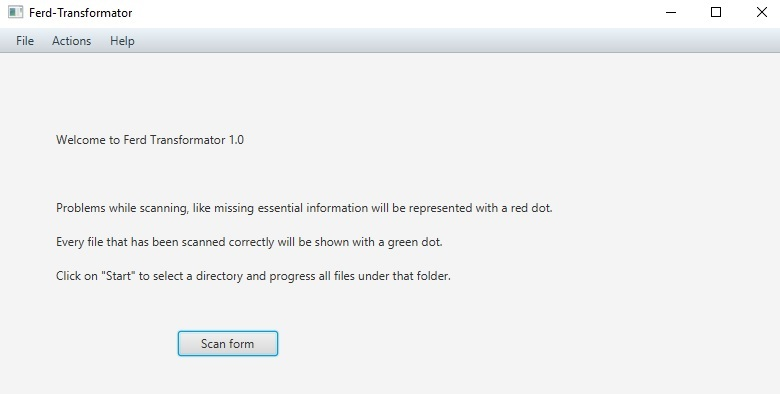
\includegraphics[width=\textwidth]{Images/GUI/startmenu.jpg}
\caption{The start page of the application \label{startmenu}}
\end{figure}

In the top there are the buttons 'File', 'Actions' and 'Help'. File enables the user to open the settings view (as discussed in \ref{sec5.7.3}) and to close the application.
Actions also contains the possibility of starting to process a form directory, as well as the search function (as explained in \ref{sec5.7.2}.
Help contains information about the application (such as version, used frameworks etc.) and links to a help document.

After the user clicked on the 'Scan form' button, a file chooser opens where the user can choose a directory where the files are. When the user has selected a directory, the application begins processing the forms under that directory.

This process can be seen in figure \ref{processingFiles}.

\begin{figure}[ht!]
\centering
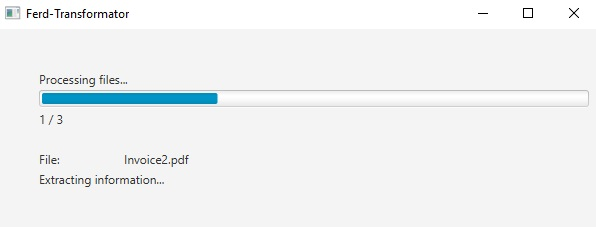
\includegraphics[width=\textwidth]{Images/GUI/processingFiles.jpg}
\caption{Processing document files \label{processingFiles}}
\end{figure}

During the extraction process, a progress bar indicates the progress of the processing of the documents. In addition to that, the current file, the file name as well as the current state is provided to give the user a possibility to estimate the remaining time.

When the process has finished and all invoice documents have been processed, a new page opens. Instead of saving all documents automatically, this way the user has the possibility to revise the documents before.
The page with the table of all revised documents is shown in figure \ref{reviseBeforeSafe}.

\begin{figure}[ht!]
\centering
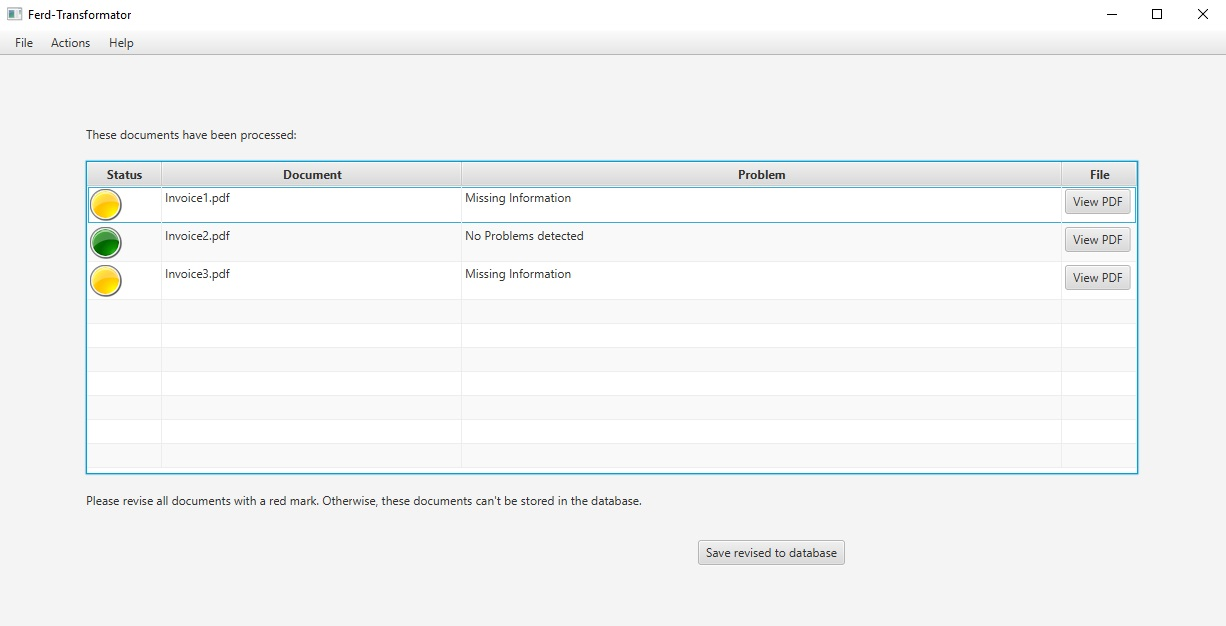
\includegraphics[width=\textwidth]{Images/GUI/reviseBeforeSafe.jpg}
\caption{Table with processed documents \label{reviseBeforeSafe}}
\end{figure}

In the first column, a coloured dots indicates possible problems with the documents. If there is a critical error in the code making it impossible to further process the document, the dot will be red. 
A yellow dot instead marks that the document has been processed successfully, but there are still issues with the documents which make it not possible to save the document at this time.
If the dot is green, these documents can instantly be saved to the database. If in doubt, the user can still access those documents too in order to check the values.

The second column contains the document name. In the third column possible problems are listed. This way the user can find out specific problems more easily.

The last column contains a button which allows the user to access the detail view of this document. There are two detail pages per document: One for basic invoice information and one for the accounting record positions.

Figure \ref{reviewElectronicInvoice} shows the first detail view.

\begin{figure}[htb!]
\centering
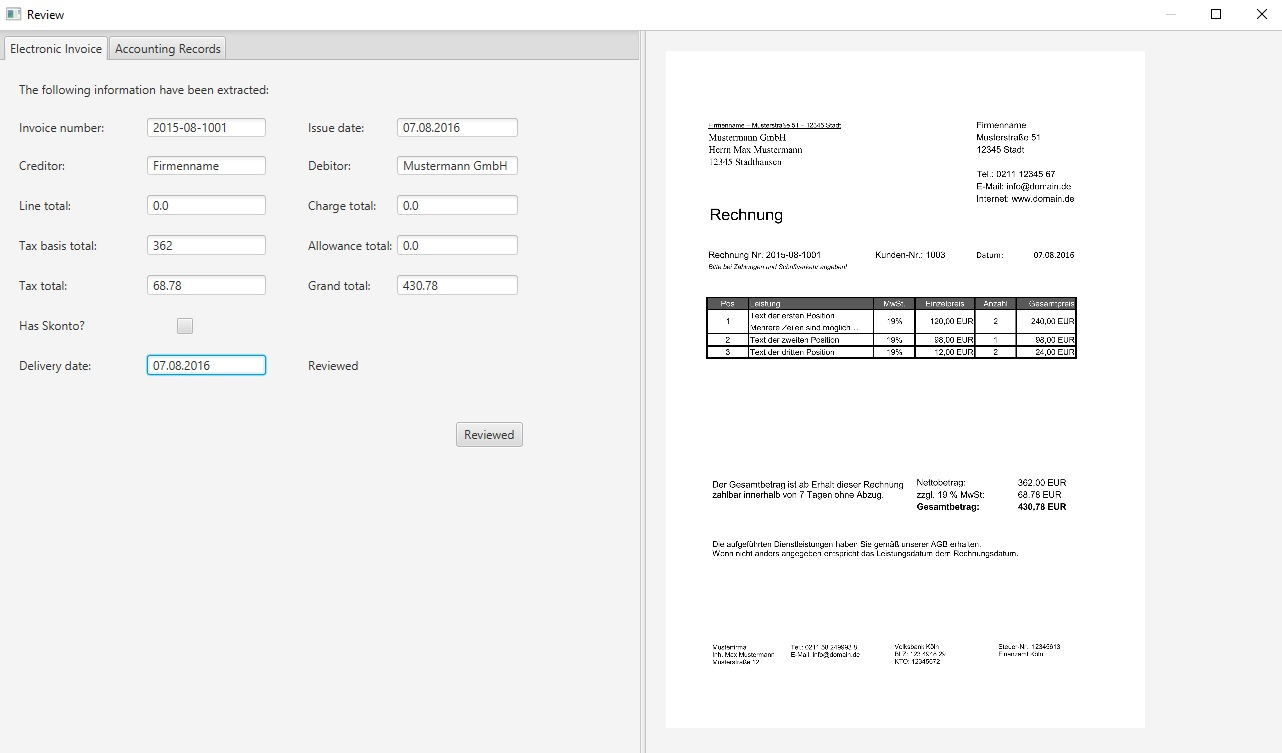
\includegraphics[width=\textwidth]{Images/GUI/ReviewElectronicInvoice.jpg}
\caption{Detail view of invoice information \label{reviewElectronicInvoice}}
\end{figure}

On the left side all the necessary information are present, while on the right side the invoice document can be seen. The user has the possibility to move the document around and zoom in and out. This is useful, if there are missing information that the user has to add in the case of missing information.

The required information on the left side are the ones required for a full conformal ZugFerd invoice of BASIC level. The amount of input fields could be enhanced in the future in order to support the COMFORT or even EXTENDED level.

All the values that have been extracted are set in to these fields. If the application was unable to extract information regarding a specific field, it will be left blank. If the user fills out the missing fields and forgets one, a validation message will be shown up, making it impossible to safe the document before filling out all fields.

If there is a Skonto applicable to the invoice, checking the checkbox 'Has Skonto?' will reveal another input field where the user is asked to provide the skonto value.

On the top left side of the image, there is also the possibility to switch between the general invoice information and the accounting records information. These information are shown in figure \ref{reviewAR}.

\begin{figure}[ht!]
\centering
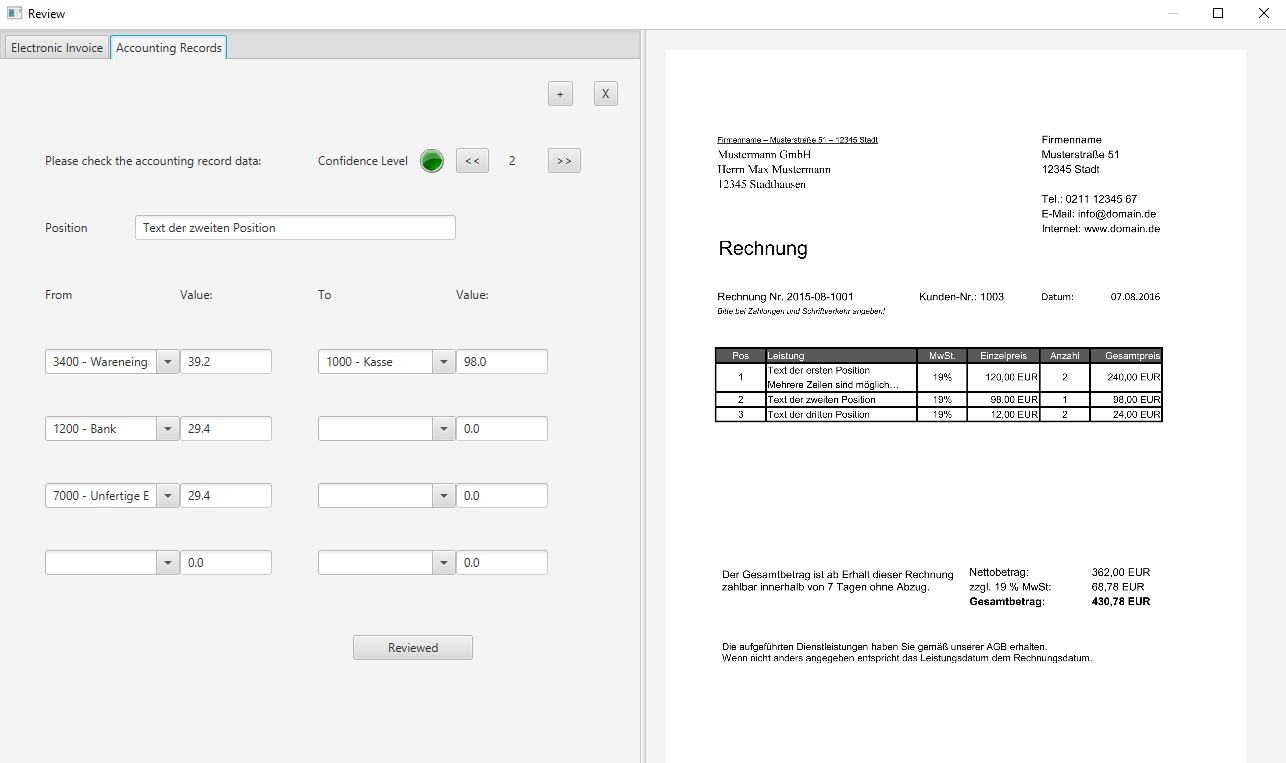
\includegraphics[width=\textwidth]{Images/GUI/ReviewAR.jpg}
\caption{Detail view of accounting record information \label{reviewAR}}
\end{figure}

This detail view looks slightly different. Positions that have been found by the application are written in the position field. But, as there can be more than position, there is the option to switch between each accounting record with the buttons in the top right of this part of the view.

For each position, there is the possibility to assign up to 8 accounts that can be involved in the accounting process (4 debit and 4 credit accounts). The amount of accounts is limited to 8, but could be enhanced in the future if there is a real need for it.

Each field of accounts can be searched for a specific name or account number, which makes working with all these accounts easier.

Note that there is a coloured dot next to the button to switch between accounting records. This dot is also an indicator how plausible the assignment is. 

In the top right corner of this side of the view there is also a '+' and a 'x' button. These can be used to add or remove accounting records as required by the user.

If the user hits the 'reviewed' button both, the invoice information as well as the accounting record information are validated. This includes:
\begin{itemize}
	\item Checking for all fields if a value is present.
	\item Calculating the values in the invoice information tab: The tax basis added by the tax total should equal the grand total value.
	\item Validating for each accounting record that:
		\begin{enumerate}
			\item There is at least one account on both, the credit and debit side
			\item An account is only used once
			\item The sum of the values of the credit side equals the sum of the values of the debit side
		\end{enumerate}
	\item Checking for empty accounts where a value has been written in
\end{itemize}

If any of these checks fail, a popup will show up and provide information which specific issues are persistent. The document can not be saved in this case. If there are no validation errors, the values are updated, the detail view closes and the user is returned to the list of the documents.

Note that the dot of the manually reviewed document has now changed from yellow to green (figure: \ref{greenAfterReview}) indicating that this document can now be saved.

\begin{figure}[ht!]
\centering

\includegraphics[width=\textwidth]{Images/GUI/GreenAfterReview.jpg}
\caption{Changing of the dot after manually reviewing the document \label{greenAfterReview}}
\end{figure}

When the user eventually clicks on 'Save revised to database', all documents with a green dot will be saved. This will also be indicated by the application with a short popup which can be seen in figure \ref{savingSuccessful}.

\begin{figure}[ht!]
\centering
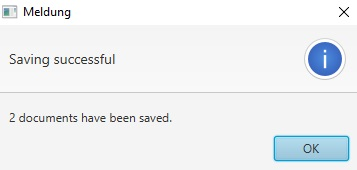
\includegraphics[width=\textwidth]{Images/GUI/SavingSuccessful.jpg}
\caption{A popup that indicates the successful saving of the documents \label{savingSuccessful}}
\end{figure}

After the saving of the document, this process is completed. The user has now the possibility to navigate over 'Actions' and either scan other documents or retrieve documents from the database. This will be covered now in the following section.

\subsection{Searching for documents in the database}
\label{sec5.7.2}

After the processing of the document, the user very likely wants to retrieve the converted document. But also older documents that once have been processed should be retrievable again.
Figure \ref{searchInDatabase} shows the possible input information. 

\begin{figure}[ht!]
\centering
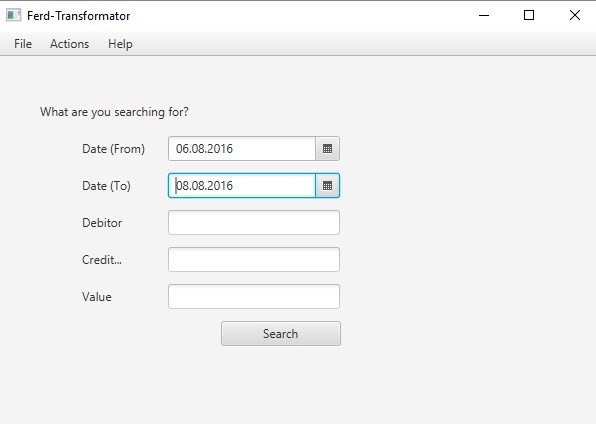
\includegraphics[width=\textwidth]{Images/GUI/SearchInDatabase.jpg}
\caption{Possible search filters for stored documents \label{searchInDatabase}}
\end{figure}

The user is able to search for invoices either on a specific date (by leaving the 'date (from)' field blank) or a timespan.
It is also possible to search for a specific creditor or debitor name or a specific value of the invoice.
None of these fields have to be filled out. It only narrows the search as a filter and will facilitate the process of retrieving the desired invoice document.

When the values have been set and the user has clicked on the button 'Search in database' a list of stored invoice documents that match the filter criteria is shown (figure \ref{searchResults}).

\begin{figure}[ht!]
\centering
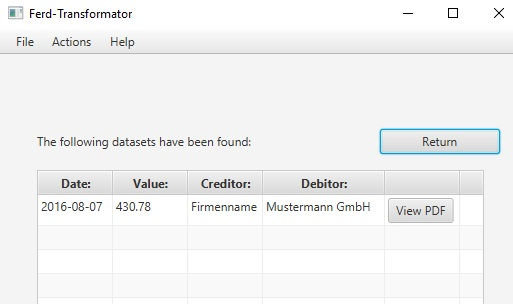
\includegraphics[width=\textwidth]{Images/GUI/SearchResults.jpg}
\caption{The results of the database search \label{searchResults}}
\end{figure}

In this list, the existing information are shown to facilitate the finding of a specific invoice. By pressing the button 'View PDF' the user is able to save the file and view it. This invoice file also contains the added electronic invoice information of the ZugFerd standard.

Pressing 'Return' enables the user to re-enter search criteria. 

\subsection{Additional settings}
\label{sec5.7.3}

To make the application flexible and adjustable to the needs of the user, we provide several possible configuration settings that can be adjusted in the settings view. This view contains of four tabs, each of them deals with settings to a specific part of the application.
Figure \ref{settings_General} shows the general settings tab. 

\begin{figure}[ht!]
\centering
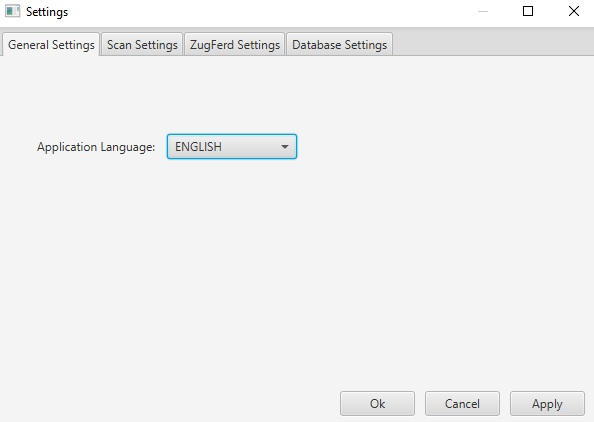
\includegraphics[width=\textwidth]{Images/GUI/settings_General.jpg}
\caption{General settings tab \label{settings_General}}
\end{figure}

This tab only contains the overall language of the application at the moment. More general settings could be added in the future. By selecting German as the application language the whole GUI will change its appeareance.

\begin{figure}[ht!]
\centering
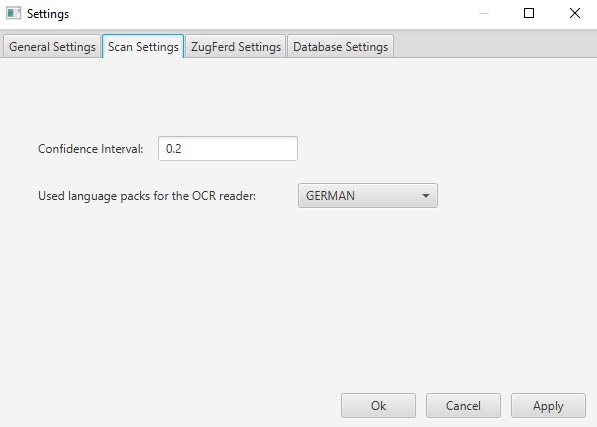
\includegraphics[width=\textwidth]{Images/GUI/settings_Scan.jpg}
\caption{Scan settings tab \label{settings_Scan}}
\end{figure}

The scan tab shows two possible options: The confidence interval and the used language packs for the OCR reader. The former value has a significant influence not only to the evaluation of the Levenshtein-Distance, but also regarding the confidence of the accounting records (which is represented as a coloured dot). A value of 0.2 means a maximum difference of 20\% or in other words: A confidence level of 80\%.

The language packs for the OCR reader are important to increase the overall OCR accuracy. If the user only uses German invoices with German words in it, the German package enables the best accuracy. But if there are other keywords or English words in general that appear in some invoices, the combination 'English and German' would deliver the best results. Pure english invoices can also be processed using the 'English' language pack.

\begin{figure}[ht!]
\centering
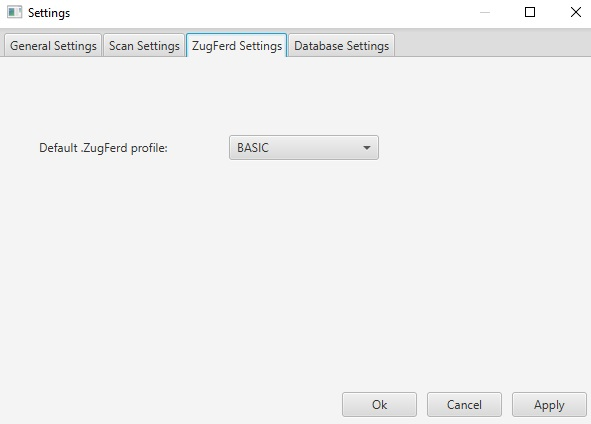
\includegraphics[width=\textwidth]{Images/GUI/settings_ZugFerd.jpg}
\caption{ZugFerd specific settings tab \label{settings_ZugFerd}}
\end{figure}

The ZugFerd tab enables the user to choose between a preferred ZugFerd level (figure \ref{settings_ZugFerd}). As of now, the application only supports the BASIC level. When the application supports Comfort or Extended level in the future, this setting would enable a different view in the invoice information detail view.

\begin{figure}[ht!]
\centering
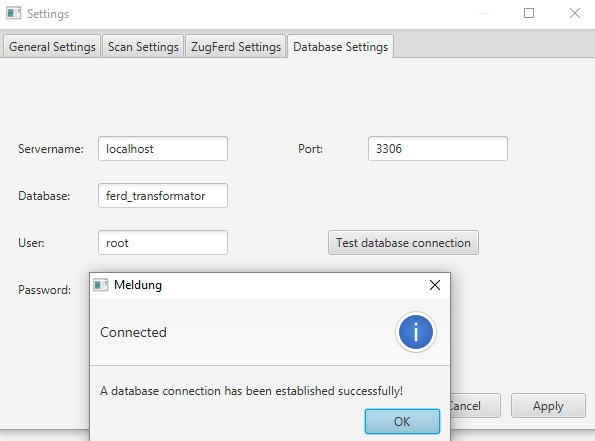
\includegraphics[width=\textwidth]{Images/GUI/settings_Database.jpg}
\caption{Database connection settings tab \label{settings_Database}}
\end{figure}

The last tab, database settings, contains several database values that can be set to a specific database. The button 'Test Connection' enables a quick connection check and returns a popup with information if the connection was successful (see also figure \ref{settings_Database}).    % (\chapter{Conclusion})
\cleardoublepage
%%%%%%%%%%%%%%%%%%%%%%%%%%%%%%%%%%%%%%%%%%%%%%%%%%%%%%%%%%%%%%%%%%%%%%%%%%%%%%%%
%
% Conclusion and outlook
% 
%%%%%%%%%%%%%%%%%%%%%%%%%%%%%%%%%%%%%%%%%%%%%%%%%%%%%%%%%%%%%%%%%%%%%%%%%%%%%%%
\chapter{Conclusion and outlook}
\label{cha6}

This final chapter concludes the thesis. First, a summary about the achievements and the resulting application is given in section \ref{sec6.1}. After that, section \ref{sec6.2} will present an outlook what future work could be done in this area. This also includes ideas or suggestions what should be changed or could be improved.

\section{Result of the application}
\label{sec6.1}

The application presented in this thesis is capable of automatic form processing. Using OCR techniques, images and pdf documents can be scanned and words extracted. Using the Hocr format, position information of specific keywords are saved and saved as cases. Those cases are used in order to improve the quality and accuracy of the algorithm over time. 

In addition to that, a Na{\"i}ve Bayes classificator is used to learn possible ways of accounting a position in regards to the different possible accounting strategies different users (or companies) can user on the same position.

As proposed in 2016, a new electronic invoice format - ZugFerd - has been published which has a high future potential. This electronic invoice format is supported by the application, as the result of the processing will be a full conformal invoice of this scheme.

\section{Future Work}
\label{sec6.2}
Even though the application is finalized and working, several improvements could be made in the future.
Each of them will be listed here, including the reasons why they should be made as well as possible ideas on how to achieve these improvements.
\begin{enumerate}
	\item Improving the accuracy of OCR: As the application is highly dependent on the successful and accurate process of OCR, improving the accuracy of the OCR process will improve the usefulness of this application in general. Hence, every action made in this direction is an advantage. There are two ideas that could be realized in the future: 
	\begin{itemize}
		\item Improving the accuracy of the Tesseract by creating an own training set based on a representative amount of invoices (especially in German) of different companies. 
		\item Exchanging the open source solution for a proprietary solution that provides a higher accuracy and / or is specialized either on invoices or German text.
	\end{itemize}
	\item Refactor the overall design of the application: Various adjustments in the application could be made to make the application more extensible in the future. The following is a list of possible changes:
	\begin{itemize}
		\item Using the strategy pattern on the OCR module: The application should be independent from which kind of OCR API it retrieves the String output. The strategy pattern would ideally lead to the possibility for the user to choose the preferred OCR reader from the settings view.
		\item Removing unnecessary or unused Business Objects, such as the Address or CorporateForm classes, since those are not used at the moment. Or instead, extend the application to make use of those classes.
		\item TO BE CONTINUED %TODO: MORE
	\end{itemize}
	\item Increase the performance of the processing step: The slowest part of the application is the process of scanning a document and extracting its information. Finding a way to speed-up this step would lead to a faster application. One idea would to parallelize the process of information retrieval with multiple documents and to make use of all processor cores the device the application runs on has.
	\item Add support for other electronic invoice standards: As of now, the application only supports the ZugFerd standard. But as stated in section \ref{sec2.3.2} before, EDIFACT has a high future potential. This also applies to the UBL standard. The more standards this application supports, the more companies can make use of it.
	\item While comparing positions we could make use of a wordnet implementation that enables us to find similar words. This way we would be able to interprete the position string in a semantic way.
\end{enumerate}   % (\chapter{})
\cleardoublepage
%%%%%%%%%%%%%%%%%%%%%%%%%%%%%%%%%%%%%%%%%%%%%%%%%%%%%%%%%%%%%%%%%%%%%%%%%%%%%%%%
%
% Conclusion and outlook
% 
%%%%%%%%%%%%%%%%%%%%%%%%%%%%%%%%%%%%%%%%%%%%%%%%%%%%%%%%%%%%%%%%%%%%%%%%%%%%%%%
\chapter{Conclusion and outlook}
\label{cha6}

This final chapter concludes the thesis. First, a summary about the achievements and the resulting application is given in section \ref{sec6.1}. After that, section \ref{sec6.2} will present an outlook what future work could be done in this area. This also includes ideas or suggestions what should be changed or could be improved.

\section{Conclusion}
\label{sec6.1}

The application presented in this thesis is capable of automatic form processing. Using OCR techniques, images and pdf documents can be scanned and words are extracted. The underlying OCR engine has been chosen by evaluating different products in order to select the most suitable one.
With implemented pre- and postprocessing steps, the accuracy of the OCR has been enhanced. Using the hOCR format that has been presented by Thomas M. Breuel\cite{Breuel07}, position information of specific keywords are saved as cases. Those cases are used in order to improve the quality and accuracy of the algorithm over time. 

In addition to that, a Na{\"i}ve Bayes classificator is used to learn possible ways of accounting a position in regards to the possible accounting strategies different users (or companies) can apply on the same position. The selection of a machine learning classifier has been made by evaluating different approaches and their accuracy. 

As proposed in 2014, a new electronic invoice format - ZugFerd - has been published which has a high future potential\cite{Ferd14}. This electronic invoice format is supported by the application, as the result of the processing will be a full conformal invoice of this scheme. The support of this format is a result of a comparison between leading and potential interesting formats in the future and the decision using predefined criteria.

The resulting converted invoices are stored in a MySQL database and can be retrieved by the user. Additional filtering allows a facilitated retrieval process. This process is also secure against SQL injections.

Several parameters of the application are customized and enables adjustments and personal preferences of the user. This also allows to further define the minimum confidence the application should have in regards to an invoice document as it classifies the document based on the confidence level. 

\section{Future Work}
\label{sec6.2}
Even though the application is finalized and working, several improvements could be made in the future.
Each of them will be listed here, including the reasons why they should be made as well as possible ideas on how to achieve these improvements.

Improving the accuracy of OCR: As the application is highly dependent on the successful and accurate process of OCR, improving the accuracy of the OCR process will improve the usefulness of this application in general. Hence, every action made in this direction is an advantage. There are two ideas that could be realized in the future: 
	\begin{itemize}
		\item Improving the accuracy of the Tesseract by creating an own training set based on a representative amount of invoices (especially in German) of different companies. 
		\item Exchanging the open source solution for a proprietary solution that provides a higher accuracy and / or is specialized either on invoices or German text.
	\end{itemize}

Refactor the overall design of the application: Various adjustments in the application could be made to make the application more extensible in the future. The following is a list of possible changes:
	\begin{itemize}
		\item Using the strategy pattern on the OCR module: The application should be independent from which kind of OCR API it retrieves the String output. The strategy pattern would ideally lead to the possibility for the user to choose the preferred OCR reader from the settings view.
		\item Removing unnecessary or unused Business Objects, such as the Address or CorporateForm classes, since those are not used at the moment. Or instead, extend the application to make use of those classes.
	\end{itemize}

Increase the performance of the processing step: The slowest part of the application is the process of scanning a document and extracting its information. Finding a way to speed-up this step would lead to a faster application. One idea would to parallelize the process of information retrieval with multiple documents and to make use of all processor cores the device the application runs on has.

Add support for other electronic invoice standards: As of now, the application only supports the ZugFerd standard. But as stated in section \ref{sec2.3.2} before, EDIFACT has a high future potential. This also applies to the UBL standard. The more standards this application supports, the more companies can make use of it.

While comparing positions we could make use of a wordnet implementation that enables us to find similar words. This way we would be able to interprete the position string in a semantic way.

Supporting other account systems besides the SKR03 could lead to a higher usefulness for companies using other account systems (such as the SKR04).   % Ausblick (\chapter{Ausblick} TEXT)
\cleardoublepage
%\include{mt08}   % Zusammenfassung (\chapter{Zusammenfassung}  TEXT)
\cleardoublepage

\chapter{InvoiceFormats}
\label{Electronic invoice formats - A comparison}

During the technologization of companies over the world, electronic invoices (also known as e-invoice) have become more and more important. E-Invoicing offers companies the possibility to improve their business processes, making invoicing faster and more efficient and enables a direct connection to other tools like ERP-Software. 

To enable companies these benefits and in order to make the communication between companies even possible a comprehensive standard has to be defined. With an invoice standard at hand, companies can use invoices from their business partners and read them into their systems (in case of B2B). 

There are several invoice standards in action at the moment. The next section will deal with the most important ones and describes them as well as pointing out the benefits and drawbacks of the format.
After that, the next section defines criteria that are relevant for the application and how to measure them.
In the last section, these criteria are applied on the formats defined in section \ref{sec2.1} and compared against each other. Eventually a decision regarding the usage of one of these formats is made.

\section{Description of leading formats}
\label{sec2.1}

\subsection{UN/CEFACT CII -> EDIFACT}
\label{sec2.1.1}

EDIFACT is a subset of standards from CEFACT regarding the electronic interchange of structured data. It is developed and maintained by the United Nations Economic Comission for Europe (UNECE). \cite{unece}

\subsection{XCBL}
\label{sec2.1.2}

\subsection{UBL OASIS}
\label{sec2.1.3}

\subsection{ZugFerd}
\label{sec.2.1.4}

\section{Definition of decision criteria}
\label{sec2.2}

While the standards defined in the section before focus on specific areas or try to combine multiple fields, this section defines the criteria that are most relevant for the application that is developed.

% Zukunftssicherheit / Aussichtsreichtum
\subsection{Future Potential}
\label{sec2.2.1}
One of the major criteria for a suitable invoice standard should be its future potential. Developing an application that deals with a standard that is not being used 10 years later does not make sense. Therefore, any standard that is going to be replaced should not be considered useful.

% Relevanz in Deutschland + Relevanz in Europa
\subsection{Relevance in Germany (and Europe)}
\label{sec2.2.2}
As this thesis is being written at a german university, the chosen standard should be relevant in Germany. Even better if it is relevant in europe as well. On the other Hand, standards that are not of interest for europe should be excluded.

% Möglichkeiten der Erweiterung in Bezug auf die Länder
\subsection{Extendability to more countries}
\label{sec2.2.3}
The possibilities of a standard to be used in other countries will also affect its importance over the next decades. Standards that only suits the requirements of one country are not important enough. The focus lies on standards with a wide (possible) range of countries to be affected, instead.

% Erweiterbarkeit des Standards allgemein bzw. was deckt er ab?
\subsection{Extendability of the standard itself}
\label{sec2.2.4}
Last but not least, the extendability of the standard itself is an important criterion. The world is changing and new requirements are coming while older ones are getting broken up. A valuable standard should be able to deal with these changes and should be extensible towards new requirements, or special requirements in specific business areas.

% Komplexität
\subsection{Complexity}
\label{sec2.2.5}
The complexity of the standard is important for this thesis too. Not only is the development of the application limited by time, but also makes a complex standard it hard to understand it and less error-prone.

\section{Comparison and decision finding}
\label{sec2.3}

\subsection{Application of the criteria}
\label{sec2.3.1}

\subsection{Decision and explanation}
\label{sec2.3.2}


\appendix
\cleardoublepage
%%%%%%%%%%%%%%%%%%%%%%%%%%%%%%%%%%%%%%%%%%%%%%%%%%%%%%%%%%%%%%%%%%%%%%%%%%%%%%%
%
% Glossary
% 
%%%%%%%%%%%%%%%%%%%%%%%%%%%%%%%%%%%%%%%%%%%%%%%%%%%%%%%%%%%%%%%%%%%%%%%%%%%%%%%

\chapter{Glossary}



B2B - Business to Business


ERP - Enterprise Resource Planning


EDIFACT - Electronic Data Interchange For Administration, Commerce and Transport


FeRD - Forum f"ur elektronische Rechnung Deutschland


SME - Small and medium enterprises


UBL - Universal Business Language


xCBL - XML Common Business Library


ZugFerd - Zentraler User Guide des Forums f"ur elektronische Rechnung Deutschland   % Glossar (\chapter{Glossar}  TEXT)
\cleardoublepage
%%%%%%%%%%%%%%%%%%%%%%%%%%%%%%%%%%%%%%%%%%%%%%%%%%%%%%%%%%%%%%%%%%%%%%%%%%%%%%%
%
% About the author
% 
%%%%%%%%%%%%%%%%%%%%%%%%%%%%%%%%%%%%%%%%%%%%%%%%%%%%%%%%%%%%%%%%%%%%%%%%%%%%%%%
\chapter{About the author}
Christoph Neubauer was born 1991 in Homburg, Germany. He made his higher education entrance qualification at the Sickingen-Gymnasium Landstuhl before he started studying Business Informatics in 2011 a the University of Applied Sciences Kaiserslautern. He finished his bachelor degree in 2015 and started the course Master Informatics at the Friedrich-Alexander University Erlangen-Nuremberg. This thesis is the final work to reach the masters degree.   % 
\cleardoublepage
\include{mt11}   % 
\cleardoublepage

%%%%%%%%%%%%%%%%%%%%%%%%%%%%%%%%%%%%%%%%%%%%%%%%%%%%%%%%%%%%%%%%%%%%%%%%%%
% Diese Datei nicht veraendern!
%%%%%%%%%%%%%%%%%%%%%%%%%%%%%%%%%%%%%%%%%%%%%%%%%%%%%%%%%%%%%%%%%%%%%%%%%%
\addcontentsline{toc}{chapter}{\listfigurename}
\listoffigures
 % Bilderverzeichnis
\cleardoublepage
%%%%%%%%%%%%%%%%%%%%%%%%%%%%%%%%%%%%%%%%%%%%%%%%%%%%%%%%%%%%%%%%%%%%%%%%%%
% Diese Datei nicht veraendern!
%%%%%%%%%%%%%%%%%%%%%%%%%%%%%%%%%%%%%%%%%%%%%%%%%%%%%%%%%%%%%%%%%%%%%%%%%%
\addcontentsline{toc}{chapter}{\listtablename}
\listoftables
 % Tabellenverzeichnis
\cleardoublepage
%%%%%%%%%%%%%%%%%%%%%%%%%%%%%%%%%%%%%%%%%%%%%%%%%%%%%%%%%%%%%%%%%%%%%%%%%%
% Diese Datei nicht veraendern!
%%%%%%%%%%%%%%%%%%%%%%%%%%%%%%%%%%%%%%%%%%%%%%%%%%%%%%%%%%%%%%%%%%%%%%%%%%
\addcontentsline{toc}{chapter}{\bibname}
\bibliography{mt}
 % Literaturverzeichnis

\bibliography{mt.bib}{}
\bibliographystyle{plain}
\end{document}
